\documentclass[french]{amu_these}

\begin{document}


	\chead{}
\pdfbookmark[0]{Page de titre}{titre}
\thispagestyle{empty}
\newgeometry{margin=2em}
% \newgeometry{left=3em,right=2em,top=2em,bottom=2em} %% marge pour la reliure en cas d'exemplaire imprimé

\begin{center}
	\begin{minipage}[c]{.5\linewidth}
		\raggedright\includegraphics[height=7em]{logo_amu_excellence}
	\end{minipage}\hfill
	\begin{minipage}[c]{.5\linewidth}
		%\raggedleft\includegraphics[height=7em]{example-image-b} %% logo cotutelle
	\end{minipage}\hfill
\end{center}

\vspace{1em}

\begin{center}
	\begin{minipage}[c]{.63\linewidth}
		\dhorline{\textwidth}{4pt}
	\end{minipage}\hfill
	\begin{minipage}[c]{.35\linewidth}
		\raggedleft\titl{NNT/NL : 2020AIXM0001/001ED000}
		% renseigner votre numéro national de thèse (NNT) et le numéro local (NL)
		% ils sont indiqués sur la page d'informations administratives de votre espace de dépôt dans le guichet de dépôt légal des thèses AMU lorque votre date de soutenance est renseignée par votre service de scolarité
		% https://depot-theses.univ-amu.fr/
	\end{minipage}\hfill
\end{center}

%\vspace{1em}

\doublespacing
\begin{flushleft}
    \titb{\HUGE\textcolor{cyanamu}{THÈSE DE DOCTORAT}}\\
	\titl{\Large Soutenue à Aix-Marseille Université}\\
	%\titl{\Large dans le cadre d'une cotutelle avec }\\
	\titl{\Large le 27 Octobre 2023}\\
\end{flushleft}
\vspace{2em}
\begin{center}
	\titsb{\Huge Pierre LECHIFFLART}\\
    \vspace{1em}
	\titm{\LARGE Exciton-phonon coupling and phonon-assisted luminescence in hexagonal Boron Nitride nanostructures}\\
\end{center}
\singlespacing

\vspace{4em}

\begin{center}
	\begin{minipage}[t]{.45\linewidth}
    	    \vspace{.5em}
        	\titb{Discipline}
        	
        	\titl{Physique et Sciences de la Matière}
        	
    	    \vspace{1em}
        	\titb{Spécialité}
        	
        	\titl{Matière Condensée et Nanosciences}
        	
    	    \vspace{2em}
        	\titb{École doctorale}
        	
        	\titl{352 PHYSIQUE ET SCIENCES DE LA MATIERE}
        	
    	    \vspace{1em}
        	\titb{Laboratoire/Partenaires de recherche}
        	
        	\titl{CINaM - Centre Interdisciplinaire de Nanosciences de Marseille / UMR 7325
        	}
	\end{minipage}\hfill
	\begin{minipage}[t]{.03\linewidth}
	    \dvertline{4pt}{-16em}
	\end{minipage}\hfill
	\begin{minipage}[t]{.52\linewidth}
	    \vspace{.5em}
    	\titb{\small Composition du jury}

	    \vspace{1em}
    	\titel{
        \begin{tabular}{p{12em} p{9.5em}}
        	Olivia PULCI & Rapporteuse \\
        	Université de Rome Tor Vergata \\
        	\\
        	Sylvain LATTIL & Rapporteur \\
        	CEA Saclay \\
            \\
            Valerio OLEVANO & Examinateur \\
        	Institut Néel, Grenoble \\
            \\
        	Aurélien MANCHON & Président du jury \\
        	Aix-Marseille Université, CINaM \\
            \\
        	Claudio ATTACCALITE & Directeur de thèse \\
        	CNRS-CINaM, Marseille \\
        \end{tabular}
        }
	\end{minipage}\hfill
\end{center}       

\vspace{2em}

\begin{center} %% logos partenaires
	\begin{minipage}[c]{.25\linewidth}
		\centering
\includegraphics[height=5em]{logo/logo-cinam} 
	\end{minipage}\hfill
	% \begin{minipage}[c]{.25\linewidth}
	% 	\centering\includegraphics[height=5em]{example-image-b}
	% \end{minipage}\hfill
\end{center}

\restoregeometry				%% page de titre

	\newpage 
\
\newpage
\chapter*{Affidavit}					
\addcontentsline{toc}{chapter}{Affidavit}
\thispagestyle{empty}
\iffalse % Déclaration sur l'honneur pour une thèse en français (inverser les \if pour une thèse en anglais)
    Je soussigné, [Prénom Nom], %% Prénom et Nom de l'auteur %%
    déclare par la présente que le travail présenté dans ce manuscrit est mon propre travail, réalisé sous la direction scientifique de [Prénom Nom], % Prénom et Nom du directeur de thèse et s’il y a lieu du co-directeur de thèse
    dans le respect des principes d’honnêteté, d'intégrité et de responsabilité inhérents à la mission de recherche. Les travaux de recherche et la rédaction de ce manuscrit ont été réalisés dans le respect à la fois de la charte nationale de déontologie des métiers de la recherche et de la charte d’Aix-Marseille Université relative à la lutte contre le plagiat.
    
    Ce travail n'a pas été précédemment soumis en France ou à l'étranger dans une version identique ou similaire à un organisme examinateur.\\
    
    Fait à [ville] le [date]
    
    \begin{flushright}\includegraphics[width=120px,height=40px]{example-image-a}\end{flushright}% signature
\fi

\iftrue % Affidavit of Honour for english thesis (invert the \if for an English thesis)
    I, undersigned, Pierre Lechifflart, %% First Name and Surname of the PhD student
    hereby declare that the work presented in this manuscript is my own work, carried out under the scientific direction of Dr. Claudio Attaccalite, %% First Name and Surname of the thesis director and if applicable of the co-thesis director
    in accordance with the principles of honesty, integrity and responsibility inherent to the research mission. The research work and the writing of this manuscript have been carried out in compliance with both the french national charter for Research Integrity and the Aix-Marseille University charter on the fight against plagiarism.
    
    This work has not been submitted previously either in this country or in another country in the same or in a similar version to any other examination body.\\
    
    Marseille, 28 August 2023
    
    \begin{flushright}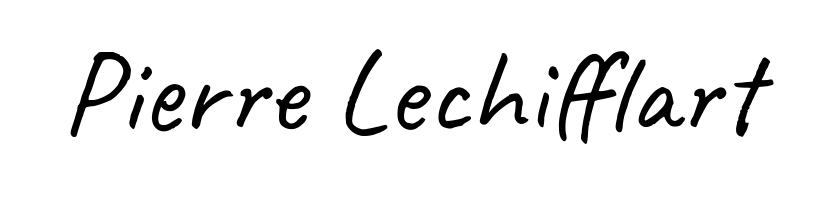
\includegraphics[width=60px,height=23px]{signaturePL.png} \ 
\includegraphics[width=46px,height=59px]{signature_pierre.png}\end{flushright} % signature
\fi

~\vfill
\begin{center}
	\begin{minipage}[c]{0.25\linewidth}
		\includegraphics[height=35px]{by-nc-nd-eu}
	\end{minipage}\hfill
\end{center}

Cette \oe{}uvre est mise à disposition selon les termes de la \href{https://creativecommons.org/licenses/by-nc-nd/4.0/deed.fr}{Licence Creative Commons Attribution - Pas d’Utilisation Commerciale - Pas de Modification 4.0 International}. % consultez les conditions de la licence cc by-nc-nd, vous pouvez appliquer une licence moins restrictive, cc by-nc-sa par exemple
				%% affidavit et licence

	\newpage
\chapter*{Liste de publications et participation aux conférences}
\addcontentsline{toc}{chapter}{Liste de publications et participation aux conférences}
\subsection*{Liste des publications réalisées dans le cadre du projet de thèse:}
\begin{enumerate}
\item \underline{Pierre Lechifflart}, Fulvio Paleari and Claudio Attaccalite. “Excitons under strain: light absorption and emission in strained
hexagonal boron nitride”. In: SciPost Physics 12 (May 2022), p. 145.
\item \underline{Pierre Lechifflart}, Fulvio Paleari, Davide Sangalli and Claudio Attaccalite. “First-principles study of luminescence in hexagonal boron
nitride single layer: Exciton-phonon coupling and the role of substrate”. In: Physical Review Materials 7.2 (Feb. 2023).
\item Michele Re Fiorentin, \underline{Pierre Lechifflart} and Fulvio Paleari, "Electronic structure and luminescence of Bernal Boron Nitride", \textit{en péparation}.
\end{enumerate}


\subsection*{Participation aux conférences et écoles d’été au cours de la période de thèse:}
\begin{enumerate}
\item Virtual school on electronic excitations in solids and nanostructures using the Yambo code, Avril 2021, en ligne
\item 17th ETSF Young Researchers Meeting, Septembre 2021, Cagliari
\item 12th Meeting on NanoScience Advances, Septembre 2021, Porquerolles
\item School : ab initio Many-body methods and simulations with the yambo code, Avril 2022, Trieste  
\item 25th ETSF Workshop, Juin 2022, Leuven
\item 18th ETSF Young Researchers Meeting, Septembre 2022, Marseille
\item Green's function methods : the next generation Workshop, Novembre 2022, Toulouse
\item GDR HOWDI annual meeting, Mai 2023, Porquerolles
\item International BN Workshop, Mai 2023, Montpellier
\end{enumerate}			%% liste de publications et participation aux conférences

	\chapter*{Résumé}
\addcontentsline{toc}{chapter}{Résumé}

%

%

\selectlanguage{french}
La présente thèse de doctorat explore l'interaction complexe entre les excitons et les phonons dans les nanostructures de nitrure de bore hexagonal (hBN) à l'aide de méthodes de calcul avancées. La thèse commence par une introduction au hBN, mettant en lumière ses propriétés uniques et son importance dans la physique de la matière condensée. 

Le chapitre 2 donne un aperçu complet du cadre théorique de pointe utilisé tout au long de la recherche, englobant la théorie de la fonctionnelle de la densité (DFT), la théorie des perturbations de la fonctionnelle de la densité (DFPT) pour les propriétés des phonons, et la théorie des perturbations à N-corps (MBPT) à travers l'approximation GW et l'équation de Bethe-Salpeter pour prendre en compte les effets collectifs électroniques et excitoniques.

Dans le chapitre 3, l'accent est mis sur le hBN massif soumis à une déformation uniaxiale, où le couplage exciton-phonon est étudié à l'aide d'une méthode de dérivation par différences finies. Cette approche reproduit approximativement les changements d'intensité de la luminescence observés lorsqu'une contrainte est appliquée au cristal. Les résultats de ce chapitre donnent des indications précieuses sur les propriétés électroniques, phononiques et excitoniques, ainsi que sur les interactions exciton-phonon dans les systèmes hBN massifs soumis à une déformation uniaxiale.

Le chapitre 4 se penche sur l'étude du hBN monocouche, en utilisant une méthode ab initio fondée sur une dérivation théorique rigoureuse des éléments de matrice du couplage exciton-phonon. En incorporant les pics directs et indirects dans les spectres de luminescence, cette méthode donne des intensités relatives détaillées, permettant une interprétation précise des mesures expérimentales publiées par différents groupes de recherche. Notamment, cette étude élimine la possibilité d'observer des répliques de phonons dans les spectres du hBN monocouche, apportant une nouvelle clarté à des interprétations auparavant ambiguës.

En outre, la thèse présente des résultats préliminaires pour le BN Bernal, un polytype de hBN avec un empilement de couches différent, présentant des gaps d'énergie directs et indirects très proches les uns des autres. Ce matériau intrigant a le potentiel d'afficher simultanément des pics directs et indirects dans les spectres de luminescence. Dans le cadre des recherches en cours qui incluent une étude numérique poussée, ce chapitre ouvre la voie à une compréhension plus approfondie des interactions exciton-phonon dans la phase Bernal du BN.

Dans l'ensemble, cette thèse de doctorat contribue de manière significative au domaine de la physique computationnelle de la matière condensée en clarifiant les phénomènes complexes de couplage exciton-phonon dans diverses nanostructures hBN. Les connaissances acquises grâce à cette étude peuvent faire progresser la compréhension et la conception de nouveaux dispositifs optoélectroniques basés sur des matériaux hBN.

\vspace{0.5cm}
Mots-clés: luminescence, phonons, excitons, couplage exciton-phonon					%% résumé

	\chapter*{Abstract}
\addcontentsline{toc}{chapter}{Abstract}
\selectlanguage{english}

The present PhD thesis explores the intricate interplay between excitons and phonons in hexagonal Boron Nitride (hBN) nanostructures through advanced computational methods. The thesis commences with an introduction to hBN, shedding light on its unique properties and relevance in condensed matter physics. 

Chapter 2 provides a comprehensive overview of the state-of-the-art theoretical framework employed throughout the research, encompassing Density Functional Theory (DFT), Density Functional Perturbation Theory (DFPT) for phonon properties, and Many-Body Perturbation Theory (MBPT) through the GW approximation and the Bethe-Salpeter equation to account for collective electronic and excitonic effects.

In Chapter 3, the focus lies on uniaxially strained bulk hBN, where the exciton-phonon coupling is studied using a finite-difference derivative method. This approach approximately reproduces the changes in luminescence intensity observed when strain is applied to the crystal. The outcomes of this chapter offer valuable insights into the electronic, phononic and excitonic properties, as well as exciton-phonon interactions in bulk hBN systems under uniaxial strain.

Chapter 4 delves into the investigation of monolayer hBN, employing an ab initio method grounded on a rigorous theoretical derivation of the exciton-phonon coupling matrix elements. By incorporating both direct and indirect peaks in the luminescence spectra, this method yields detailed relative intensities, enabling an accurate interpretation of experimental measurements published by different research groups. Notably, this study eliminates the possibility of observing phonon replicas in the spectra of monolayer hBN, providing new clarity to previously ambiguous interpretations.

Furthermore, the thesis offers preliminary results for Bernal BN, a polytype of hBN with a different layer stacking, featuring closely situated direct and indirect energy gaps. This intriguing material holds potential for displaying simultaneously both direct and indirect peaks in luminescence spectra. As part of ongoing research that includes deep numerical studies, this chapter paves the way for a deeper understanding of exciton-phonon interactions in Bernal BN structures.

Overall, this PhD thesis contributes significantly to the field of computational condensed matter physics by unraveling the complex exciton-phonon coupling phenomena in various hBN nanostructures. The insights gained from this study have the potential to advance the understanding and design of novel optoelectronic devices based on hBN materials.

\vspace{0.5cm}
Keywords: luminescence, excitons, phonons, exciton-phonon coupling

				%% abstract

	\chapter*{Acknowledgments / Remerciements}
\addcontentsline{toc}{chapter}{Acknowledgments / Remerciements}

First I would like to thank the board of Doctoral School 352 that granted me this PhD funding, Andrea Marini for hosting me one week in Rome, funded by the Cost Action TUMIEE, Daniele Varsano and HPC Europa3 for allowing me a 2-month visit in Modena.

I would like to thank my supervisor Claudio for his constant support, his availability, for giving me the freedom to study the things I wanted and for his wise decisions that helped me to become a scientist. Un ringraziamento speciale per il tempo che hai dedicato alla revisione di questo manoscritto.


I would like to thank Khaoula Boukari and Andres Saul for the management and maintenance of the computer cluster \textit{Rosa} which was an undeniable advantage for this PhD work.

I thank the TSN department as a whole for scientific discussions and at large, everyone who I discussed about science with and who sated my hunger for understanding, Elena Cannuccia, Adrien Rousseau, Thibaut Sohier, Pedro Melo, Martino Silvetti, Matteo Zanfrognini, Riccardo Reho.

I thank the people I met in CINaM and who became my friends : Anna, Petr, Clémence, Céline, Alex, Julien, Diego, Ilan, Rajarshi, Guillem, Djouher, Mathilde, Kostis, Tarik, Gaëlle, Giorgia, Luigi,  Mohit, Vyshnav. You contributed to brighten the sometimes gloomy days. 

I thank Vitaly, Laura, Miguel and Kalyani for their help in the organization of YRM 2022 which was quite an experience, Véronique, Régine, Lydia, Cindy, Sabina for the precious administrative help, and Christophe for the budgetary rescue.

I thank Marine Baujon for helping me manage things that felt bigger than me at times.

I thank everyone for good times in Marseille and elsewhere Sam, Yann, Jonathan, Pavlo, Vasile, Thaïs, Simon, Inès.

Merci à mes proches qui donnent un sens à tout ceci. Jules, Pieric, Valentin, Yann, merci de votre soutien indéfectible, vous êtes des amis formidables.

Un simple merci ne suffirait pas pour exprimer ma gratitude envers mes parents et ma famille. Merci Maman et Papa pour m'avoir toujours soutenu et exprimé votre fierté. Merci Baptiste et Maxime d'être des frères admirables. Merci Côme et Thaïs de bien vouloir jouer avec moi.				%% remerciements

    \microtypesetup{protrusion=false}	%% désactive la protrusion (TOC LOFT GLS)
	\tableofcontents					%% TOC
	\listoffigures						%% LOF
	\listoftables						%% LOT
	\printglossary[						%% acronymes
		type=\acronymtype,
		title={List of acronyms},
		toctitle={List of acronyms}
		]
	\printglossary[						%% glossaire
		title={Glossary},
		toctitle={Glossary}
		]
	% \printglossary[						%% nomenclature
	% 	type=notation,
	% 	title={Nomenclature},
	% 	toctitle={Nomenclature}
	% 	]
    \microtypesetup{protrusion=true}	%% rétabli la protrusion

	\ohead{\leftmark\Ifstr{\rightmark}{\leftmark}{}{ -- \rightmark}}	%% place le chapitre et la partie en en-tête

	\chapter*{Introduction}
\addcontentsline{toc}{chapter}{Introduction}
Generalities about hBN \\
We could compute phonon-assisted absorption but the phonon satellites are very small wrt to the main peaks so when they overlap, they are not visible.\\
Theory of phonon-assisted optics : it exists. For instance, Williams-Lax theory that treats lattice-dependent band features and phonon-assisted transitions 
There is also Hallen-Bardeen-Blatt and Heine-Cardona but I don't know too much about them.
Besides, some models of exciton-phonon coupling exists also, some specifically for luminescence, but they are computationally expensive for real materials.
==> there is a need for exciton-phonon coupling and phonon-assisted optics from first principles. In chapters 2 and 3, two different approaches are presented in section \textcolor{red}{ref to sections}. The first one consists in calculating the response function correction due to exciton-phonon coupling from finite differences, by displacing atoms in supercells. The second one is a more general approach based on \acrshort{MBPT}, in which a dynamical correction induced by electron-phonon coupling is added as a perturbation to the Bethe-Salpeter kernel. Thanks to this \textit{ab initio} framework, the scattering of every exciton with every phonon mode can be computed, over the whole Brillouin Zone. These calculations are done in the unit cell.
Both approaches allow to compute the exciton-phonon coupling. Then, the absorption can be obtained after post-processing of a standard \acrshort{BSE} calculation. To obtain the luminescence spectra, we use the van Roosbroeck -- Shockley relation for both cases.
Exciton-phonon in hBN are not only possible, but likely due to strong electron-phonon coupling. Verified experimentally by the External Quantum Efficiency comparable to direct gap materials.
%
%
%
ETSF webinar of Fulvio
indirect bandgap only; we can write the response function with derivatives of the response function because we consider only phonon-assisted transitions; need supercells
converge the displacement so that it is the smallest possible
PLE (propto absorption) or absorption and PL are not symmetric, as expected for direct gaps
the minimum exciton at T is the degenerate dark state at Gamma which splits
for absorption, the bright exciton overlaps with the phonon replicas and it is so bright that we don't see them 

	\chapter{ State of the art theory}
\chaptertoc{}

\section{Introduction on the many-body problem}
%generalities on theories that are the building blocks of our workflows
%what is ab initio
The system of interacting electrons and nuclei in a material is described by the following Hamiltonian :
\begin{align}
	\hat{H} = &- \sum_I \frac{\hbar^2}{2 M_I} \nabla^2_I + \frac{1}{2} \sum_{I\neq J} \frac{Z_I Z_J e^2}{\left| \RR_I - \RR_J \right|} \nonumber \\
	&- \frac{\hbar^2}{2m_e} \sum_i \nabla^2_i + \frac{1}{2} \sum_{i\neq j} \frac{e^2}{\left| \rr_i - \rr_j \right|} - \sum_{i,I} \frac{Z_I e^2}{\left|\rr_i - \RR_I \right|}
\end{align}
where capital indices refer to nuclei and lowercase indices refer to electrons. $Z_I$, $M_I$ and $\RR_I$ are the atomic number and the position in real space of nucleus $I$.
The terms on the first line are the kinetic energy of the ions and the ion-ion interaction, respectively.
%atomic units
%Born-Oppenheimer

\section{Density Functional Theory}
% This theory is vastly used in solid-state physics and quantum chemistry, and it is the starting tool to compute structural and electronic properties of our systems.
The idea behind \gls{DFT} is to replace the real system of interacting electrons by an auxiliary system of non-interacting particles evolving in an effective potential.

\gls{DFT} is a theory of the interacting electron system and is based on the work of Hohenberg and Kohn who stated and proved two fundamental theorems. \cite{hohenberg1964} The first one ensures there is a one-to-one correspondance between the electronic density and the external potential acting on the system. The second theorem states that the total energy of the system is a functional of the electronic density.
The total energy of a system of interacting electrons is written as :
\be
	E = \expval{\hat{H}}{\Psi} = \expval{\hat{T} + \hat{V}_{ee} }{\Psi} + \int d\rr v_{ext}(\rr)n(\rr)
\ee
By virtue of the Hohenberg and Kohn theorems, the total energy is a functional of the density and can be written as :
\be
 	E_{HK}[n] = F_{HK}[n] + \int d\rr v_{ext}(\rr)n(\rr)
	\label{eq:E_HK}
\ee
where $F_{HK}[n] = \la \hat{T} \ra + \la \hat{V}_{ee} \ra$ is a universal functional of the density, \emph{ie} the dependence on $n$ of the functional is the same for all systems. The ground-state energy $E = E_0$ is the minimum of the energy functional at the ground-state density $n=n_0$. To be able to compute these quantities, Kohn and Sham reformulated the problem into an auxiliary system of non-interacting particles, that has the same density as the real system. This reformulation is particularly helpful because it is possible to compute analytically the kinetic energy term. The only subtlety is that one needs to use the density \emph{matrix} rather than the electronic density, that is defined as the expectation value of the density operator $\hat{\delta}(\rr) = \sum_i^{N_{e}} \delta(\rr - \rr_i)$ :
\begin{align}
\begin{split}
	n(\rr) &= \int d^3r_1 ... d^3r_{N_{e}} \Psi^*(\rr_1,...,\rr_{N_{e}})
	\hat{\delta}(\rr) \Psi(\rr_1,...,\rr_{N_{e}}) \\
	&= N_{e}\int d^3r_2 ... d^3r_{N_{e}} \left| \Psi(\rr,\rr_2...,\rr_{N_{e}})\right|^2
\end{split}
\end{align}
This is related to the probability density of finding a particle at position $\rr$.
The expression for the total energy functional in \eqref{eq:E_HK} can be rewritten as :
\be
	E_{KS}[n] = T_{ip}[n] + \int d\rr v_{ext}(\rr)n(\rr) + E_H[n] + E_{XC}[n]
\ee
where $T_{ip}$ is the kinetic energy of the independent particles with density $n$, $E_H$ is the Hartree energy, which is the classical electrostatic interaction :
\be
	E_H = \int n(\rr')n(\rr)
	\label{eq:E_Hartree}
\ee
and $E_{XC}$ is the exchange-correlation energy defined as :
\be
	E_{XC}[n] = T
\ee
difference between the exact kinetic energy and $T_{ip}$ plus
contains quantum effects of exchange and correlation of fermions


	\chapter{Hexagonal Boron Nitride under strain}
\chaptertoc{}

\textit{This chapter is partly based on our publication Ref. \cite{lechifflart2022excitons}. Some of the text and figures contained in this Chapter are adapted from this reference.}

%
\section{Introduction and experimental motivations}
\textcolor{red}{Do you think I should put this in the Introduction chapter ?}
Strain is a powerful tool to engineer electronic and optical properties of materials. It is possible to modify the electronic dispersion of strained crystals, in particular to modify the conduction band minima and the valence band maxima, even leading to a direct to indirect bandgap transition, as it was shown for Germanium \cite{hoshina2009first,cheng2010strain} and more recently for transition metal dichalcogenides.\cite{desai2014strain,choudhary2020shear,frisenda2017biaxial} Regarding hBN, the effect of strain on vibrational properties was investigated experimentally in exfoliated hBN with various thicknesses,\cite{androulidakis2018strained} while theoretically biaxial tensile strain was considered for the mono- and bilayer h-BN \cite{yang2013distorted,fujimoto2016band} as well as its role on hexagonal boron nitride quantum emitters.\cite{tabesh2021strain} But little is known about the effect of strain on the optical properties of bulk h-BN, which are the simplest mean to characterize this material. \\
A recent experiment showed a remarkable modification of the cathodoluminescence spectrum of hBN under strain. \cite{schue2017proprietes} In this experiment Léonard Schué, from the group of Julien Barjon, suspended a nanosheet of hexagonal Boron Nitride over a trench carved out from an SiO$_2$ substrate. The nanosheet is about 100 nm thick and curves under the effect of gravity, as illustrated in Fig. \ref{fig:exp_strain}(a), and was imaged by \acrfull{AFM} (Fig. \ref{fig:exp_strain}(b)).
\begin{figure}[tbp]
	\vspace{0.2cm}
	\setcapindent{2em}
	\centering
	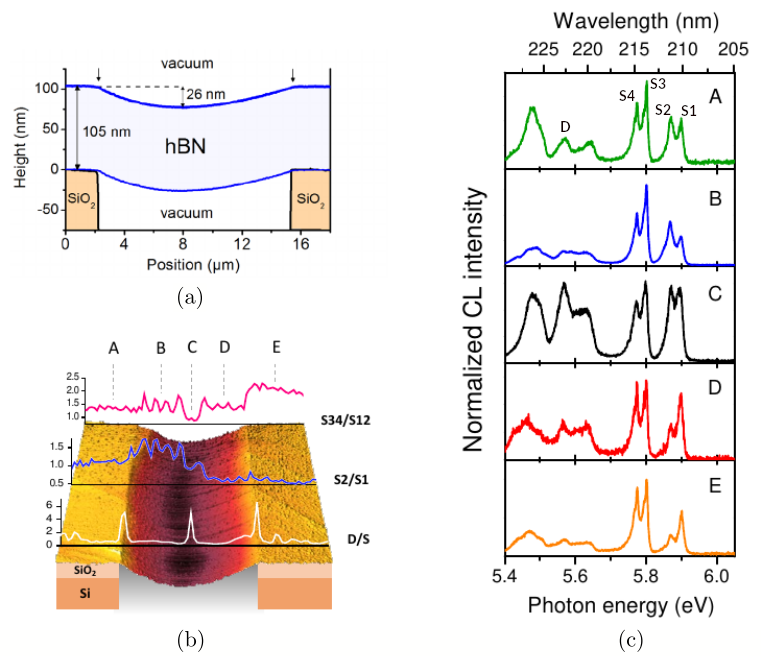
\includegraphics[width=0.7\textwidth]{exp_strain.png}
	\caption{(a) Sketch of the deposited hBN nanosheet on the trench. (b) AFM profile and relative intensity ratios of different emission peaks with respect to spatial region. (c) Cathodoluminescence intensity measured on different regions of the sample. Courtesy of Léonard Schué and Julien Barjon}
	\label{fig:exp_strain}
\end{figure}
When measuring the cathodoluminescence spectra at different positions on the sample, one can see that the intensity ratios between different peaks are varying. Their interpretation is that the deformation of the sample induces uniaxial (compressive) strain, perpendicular to the trench. This strain could have an effect on the recombination process of excitons or their scattering with phonons, leading to a change in the luminescence intensity. The measure an intensity ratio between the S1/2 and the S3/4 peaks coming from $\approx 4$ at equilibrium to almost 1 at the bottom of the trench. We try to simulate this phenomenon and use a method to reproduce the phonon-assisted luminescence from first-principles.


%
\section{Structure and phonons}
In order to simulate the hBN sample in suspension, we consider an infinite bulk crystal under uniaxial strain. In the experiment, the beam of electron penetrates only on the upper part of the nanosheet, where the strain is compressive. However for the first steps of the computational workflow, we study a range of strain including both stretching and compression around the equilibrium structure.
First, we obtain the strained structure by taking an orthorombic cell of the pristine crystal, larger than the hexagonal unit cell. Because it has three orthogonal lattice vectors, the orthorombic cell is more suited for the application of a uniaxial strain. To do so, we simply alter the length of one cell vector, up to an arbitrary length corresponding to a value of strain. We studied different strain values, in an interval going from a $+2.5\%$ to a $-2.5\%$ variation of the equilibrium length. In this work we applied strained in the armchair direction, the one parallel to the B-N bond. 
\begin{figure}[tbp]
	\vspace{0.5cm}
	\setcapindent{2em}
	\centering
	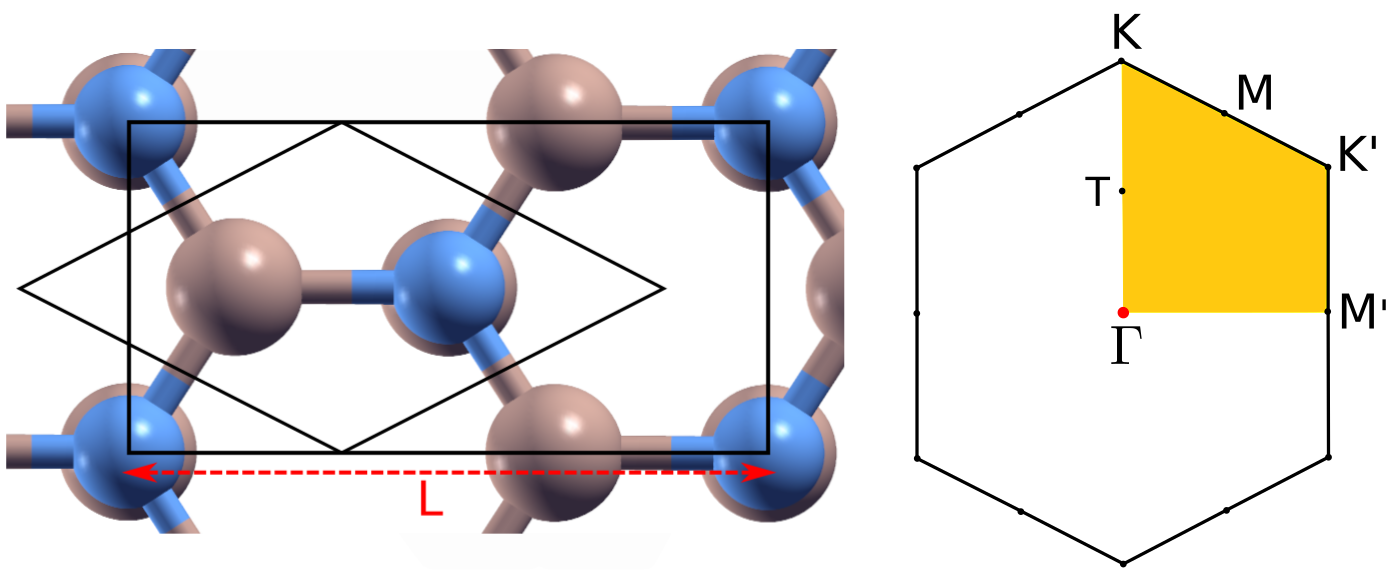
\includegraphics[width=0.8\textwidth]{AppB_structure_BZ.png}
	\caption{Left : visualization of the strained crystal and the orthorombic and pseudo-hexagonal unit cells. Right : corresponding strained Brillouin Zone. The dotted line is the shape of the equilibrium BZ. The yellow zone is the area enclosed by the high-symmetry points we used to plot dispersions.}
	\label{fig:strain_BZ}
\end{figure}
After setting the length of the cell to the desired length corresponding to a strain value, we let the atom positions and the other two cell vectors relax, using a damped molecular dynamics algorithm where the forces acting on the atoms are computed in \acrshort{DFT} using the Hellmann--Feynman theorem. This procedure in implemented in the \qe ~suite.\cite{giannozzi2009quantum,giannozzi2017advanced} More computational details can be found in Appendix \ref{app:comp_par_strain}. We found that once the two cell vectors orthogonal to the strained one are relaxed, their length vary linearly with the strain.\\
Once we have the relaxed strained orthorombic cells, we want to construct a pseudo-hexagonal unit cell containing only four atoms. This way, we can compare the structures obtained for different strain values with the equilibrium structure in a consistent way and proceed with the calculation of electronic and optical properties. To construct the pseudo-hexagonal cells from the strained orthorombic ones, we followed the procedure described in Appendix \ref{app:ortho2hex}. We computed the phonon-related properties using \acrshort{DFPT} in the four-atom strained cells. In the strained crystal, whatever the value of strain, the 120\textdegree~ rotational symmetry is broken and this makes the \MM~and \KK~points in the \acrshort{BZ} inequivalent to the \MM' and \KK' points. The path between high-symmetry points containing all four of these points is drawn in yellow in Fig. \ref{fig:strain_BZ}.
The resulting phonon dispersions are shown in Fig. \ref{fig:strain_phonons}, for three strain values : a $+2.5\%$ stretch, a $-2.5\%$ compression and the equilibrium one.
\begin{figure}[tbp]
	\vspace{0.5cm}
	\setcapindent{2em}
	\centering
	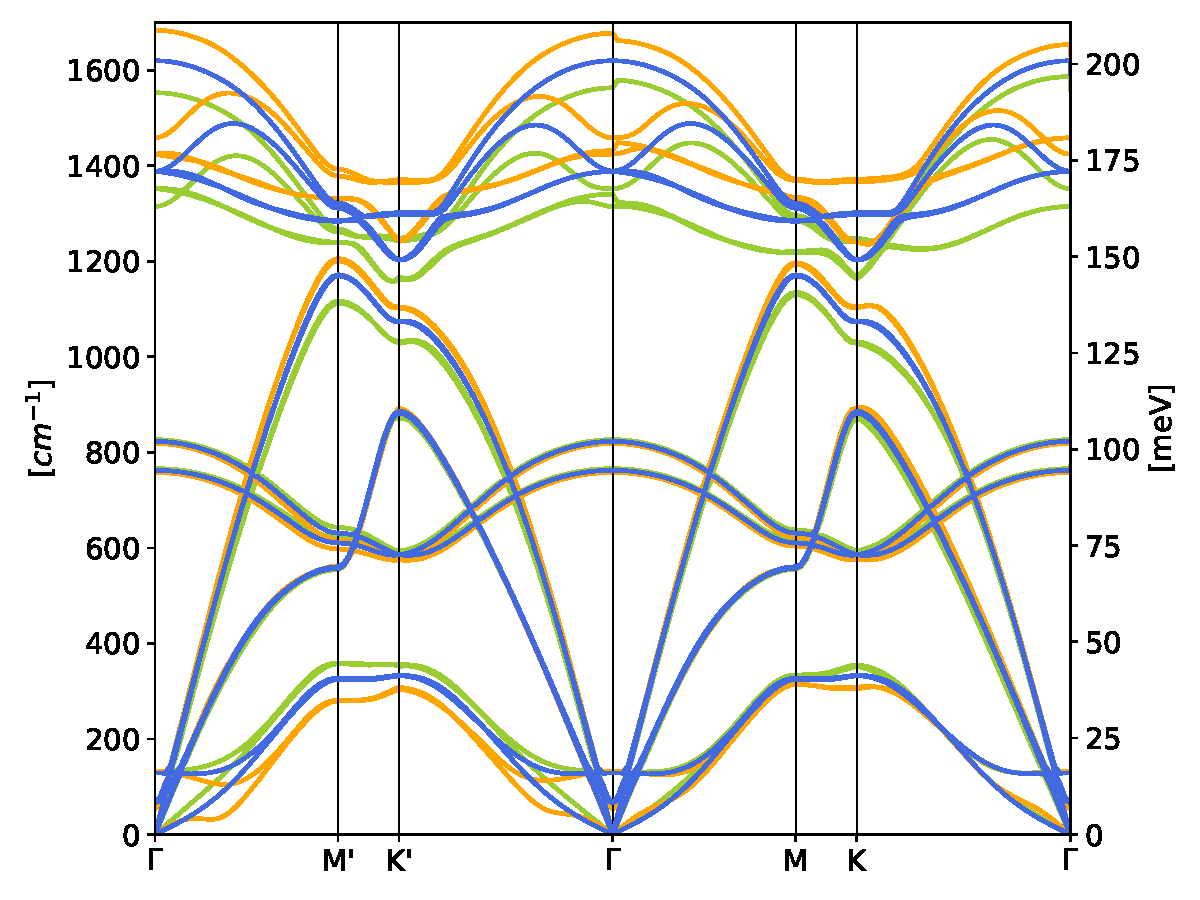
\includegraphics[width=0.8\textwidth]{strain_ph.pdf}
	\caption{Phonon dispersion versus uniaxial strain. Blue lines are at equilibrium, green lines at 2.5\% stretch and orange lines at 2.5\% compression.}
	\label{fig:strain_phonons}
\end{figure}
For the unstrained dispersion we can notice the splitting of the highest branch at $\Gamma$ with the two branches below. This is the LO-TO splitting mentionned in Sec. \ref{sec:DFPT}.

We found that the optical modes (the branches with the highest energies) are the most affected by strain. With compressive strain, their frequencies are increased at all $\qq$ points and they are decreased for tensile strain. We also observe the splitting of the E$_{2g}$ modes, whose frequencies are degenerate at $\Gamma$ just below 175 meV or 1400 cm$^{-1}$ for the unstrained structure. They split as soon as a strain is applied. This is in agreement with Raman measurements and previous calculations.\cite{blundo2022vibrational,androulidakis2018strained} It is also interesting to notice that depending on the direction along which the $\Gamma$ point is approached, the splitting of the two E$_{2g}$ modes has different magnitudes. 

On the mid-energy range of the dispersion, the LA, TA and TO modes are not very affected by strain. This will be important in the discussion about luminescence in the following.

On the lower frequency end, the acoustic modes are affected in an opposite way. Under compression, their frequencies are decreased and increased under stretch. The orange curve shows a softening of the lowest branch close to $\Gamma$. We noticed that increasing the value of compressive strain leads to giving imaginary frequencies. This happens when the geometry is unstable. Then the second derivative in Eq. \eqref{eq:IFC_matrix} is negative and the eigenvalues $\omega^2$ in Eq. \eqref{eq:ph_evprob} are negative. We did not investigate this instability caused by compression, since the range of strain we are interested in is not above $+2.5\%$ of strain. Nonetheless, the phonon dispersions show that our systems are stable in the range of strain considered.

%
\section{Electronic structure}
After computing the Kohn-Sham eigenvalues in \acrshort{DFT}, we performed a one-shot G$_0$W$_0$ calculation to compute the quasiparticle corrections using the \yambo code. We found that these corrections are a rigid shift in energy of the KS eigenvalues over the whole \acrshort{BZ}. 
\begin{figure}[tbp]
	\vspace{0.5cm}
	\setcapindent{2em}
	\centering
	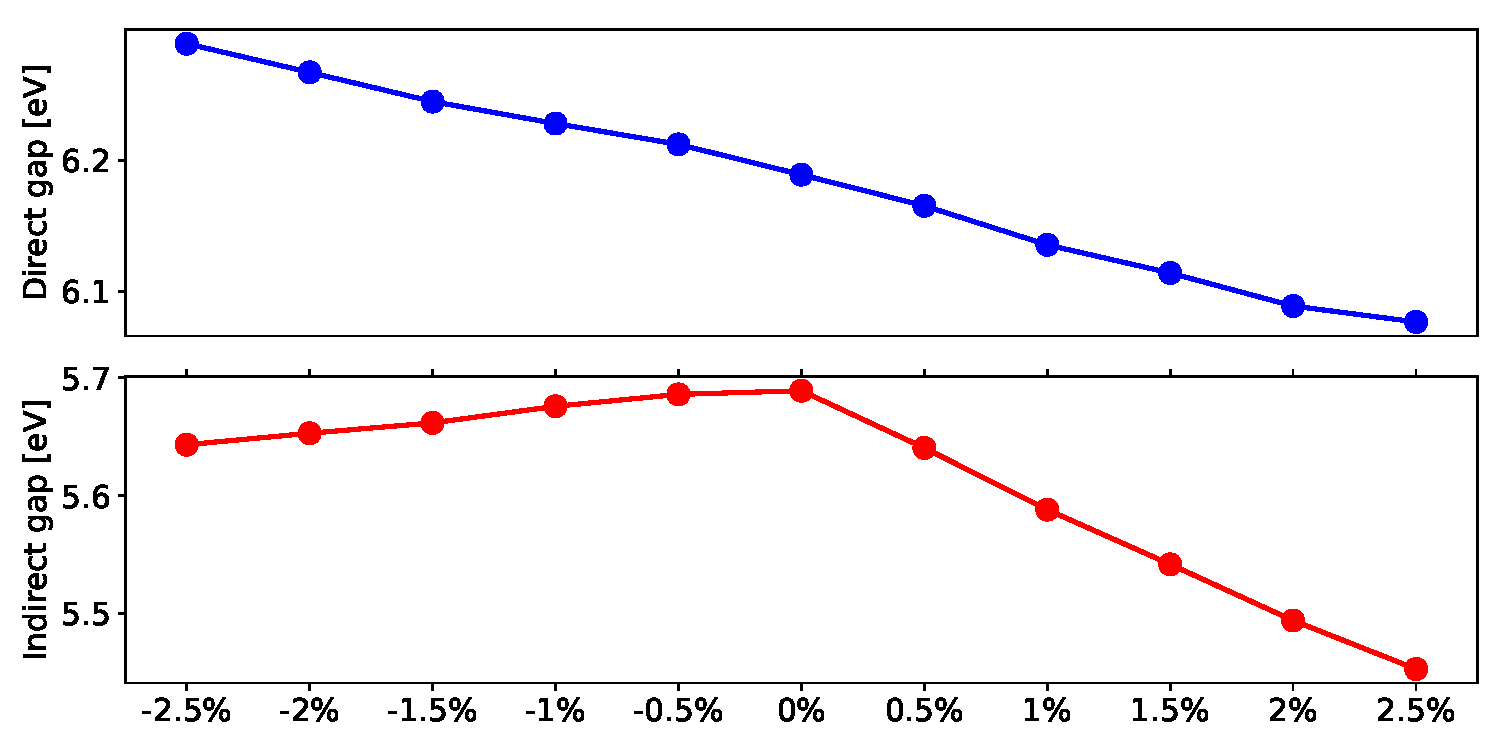
\includegraphics[width=0.8\textwidth]{strain_gw_gaps.pdf}
	\caption{Quasiparticle corrections to the direct and indirect bandgaps at the G$_0$W$_0$ level with respect to strain.}
	\label{fig:strain_gw_gaps}
\end{figure}
In Fig. \ref{fig:strain_gw_gaps} we report the variation of the direct gap (at \MM) and of the indirect gap (between \KK~and \MM) with respect to strain. The direct gap has decreases linearly with increasing relative values of strain, while the indirect gap is maximal for the unstrained system and decreases both for compression and stretch.

The electronic dispersions along the path showed above are plotted in Fig. \ref{fig:strain_eldisp} for the two maximally strained systems and for the unstrained one. 
\begin{figure}[tbp]
	\vspace{0.5cm}
	\setcapindent{2em}
	\centering
	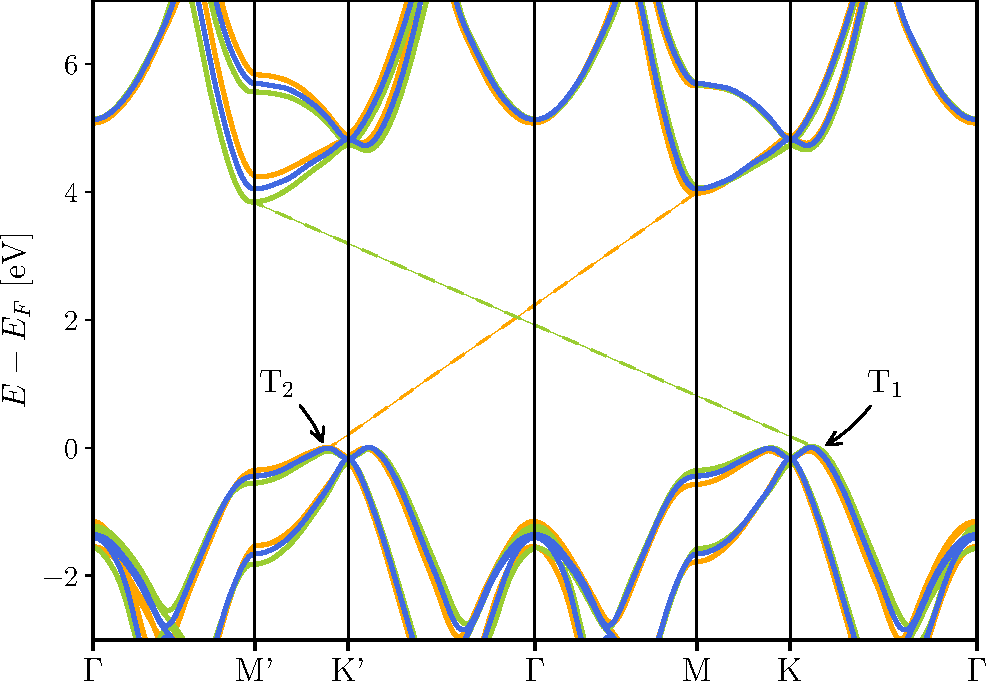
\includegraphics[width=0.6\textwidth]{strain_bands_qgaps.pdf}
	\caption{Details of the electronic band structure under the maximum
	stretch and compression considered in the manuscript. Blue lines are at equilibrium, green lines at +2.5\% stretch and orange lines at -2.5\% compression. We report also the location of the new indirect gaps in the two cases. Notice that at equilibrium all indirect transitions between the different \KK~ and \MM~ points are equivalent.}
	\label{fig:strain_eldisp}
\end{figure}
At equilibrium, the direct gap is located between states with a momentum close to \KK. The indirect gap is between a point close to \KK~for the valence band and the \MM~point for the conduction band. As discussed above, strain breaks one of the symmetries of the crystal and this effect is visible on the dispersions at high-symmetry points. Under compression, the conduction band is shifted down at \MM~while it is increased at \MM'. This trend is reversed under stretch. Hence, the conduction band minimum is at \MM~for the compressed crystal and at \MM' for the stretched crystal. 
These variations can be explained in term of the variation of the orbital properties. 
\begin{wrapfigure}{r}{0.41\textwidth}
	\vspace{-16pt}
	\setcapindent{1em}
	\centering
	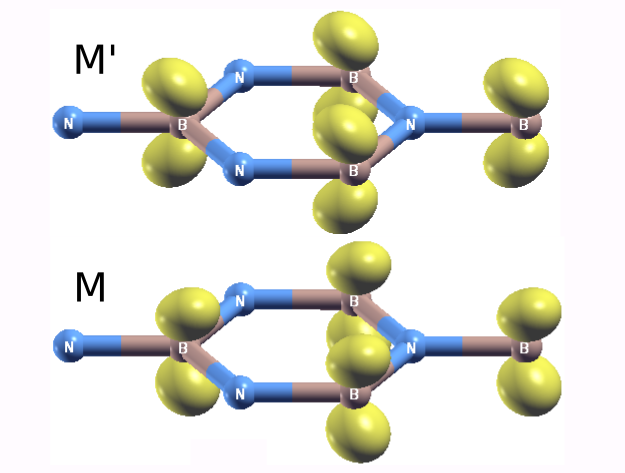
\includegraphics[width=0.4\textwidth]{M_and_M_prime.png}
	\caption{$\pi^*$ atomic-like orbitals of the conduction band minima on one of the layers for a compression of 0.5\%. At \MM', the components of the wavefunctions are oriented along the compressed B-N bond. At \MM, they are oriented along one of the other bonds.}%\textcolor{red}{Rajoute des flèches pour montrer le strain.}}
	\label{fig:WF_strain}
\end{wrapfigure}
The $\pi^*$ atomic-like orbitals at \MM~and \MM' have a different shape, as illustrated in Fig. \ref{fig:WF_strain} for a compression of 0.5\%. While they are degenerated in energy for the unstrained crystal, this degeneracy is lifted due to the symmetry breaking. The state with orbital components along the strained bond is the one whose energy changes with strain at \MM'. These orbitals are dependent on the interlayer interactions, which in turns depends on the interlayer distance. This distance varies linearly with the strain applied to the system in our relaxation process. This explains the splitting of the bands induced by strain at the \MM' point.

The valence states around \KK~and \KK' are only slightly changed in energy. This can be explained because the orbitals corresponding to these states are protected from interlayer interactions by symmetry, as shown in the theoretical study of Ref. \cite{kang2016unified}. There is nonetheless a slight change in energy, which causes the valence band maximum to be located at the point called \textbf{T}$_2$ under compression and at \textbf{T}$_1$ under stretch. %\textcolor{red}{change the names either of these points OR of the T point in the BZ scheme}. 
The minimal indirect gaps are indicated by the dotted lines in Fig \textcolor{red}{Fig5} for compressive and tensile strain.

%
\section{Excitons and absorption}
On the low-energy end of the excitonic spectrum (in the sense of linear algebra) of bulk \acrshort{hBN}, we find two pairs of degenerate excitons. The splitting between the pairs is caused by the interlayer interactions and is called the Davydov splitting.\cite{paleari2018excitons} The two pairs transform differently under inversion operation (\textit{i.e.} taking $\rr \to -\rr$ or $\kk \to -\kk$). The lowest pair is even for inversion symmetry, which means it is dark in absorption. The second lowest pair instead is odd for inversion symmetry and thus bright. \textcolor{red}{I have to explain what dark and bright is in chapter 1} 
Note that this is true for one-photon absorption, at the linear response level. In non-linear optics, for instance two-photon absorption, the dark and bright characters are reversed. \\
The 120$\textdegree$ rotation symmetry breaking induced by uniaxial strain has an effect on the degeneracy of the Davydov pairs. First, looking at the energies of the four lowest excitons at $\Gamma$, as displayed in panel $(a)$ of Fig. \ref{fig:exc_abs_vs_strain}, we see that the energies are split, both for compression and stretching. 
These changes in energy are mainly due to the change in electronic gap reported in the above section. Indeed, they follow the same linear trend as the strain value increases and are of the same magnitude, about $\pm 0.1$ eV. We could also verify that the binding energies of the direct excitons remain approximately constant on the strain range considered, varying only by 10 to 15 meV.
\begin{figure}[tbp]
	\vspace{0.2cm}
	\setcapindent{2em}
	\centering
	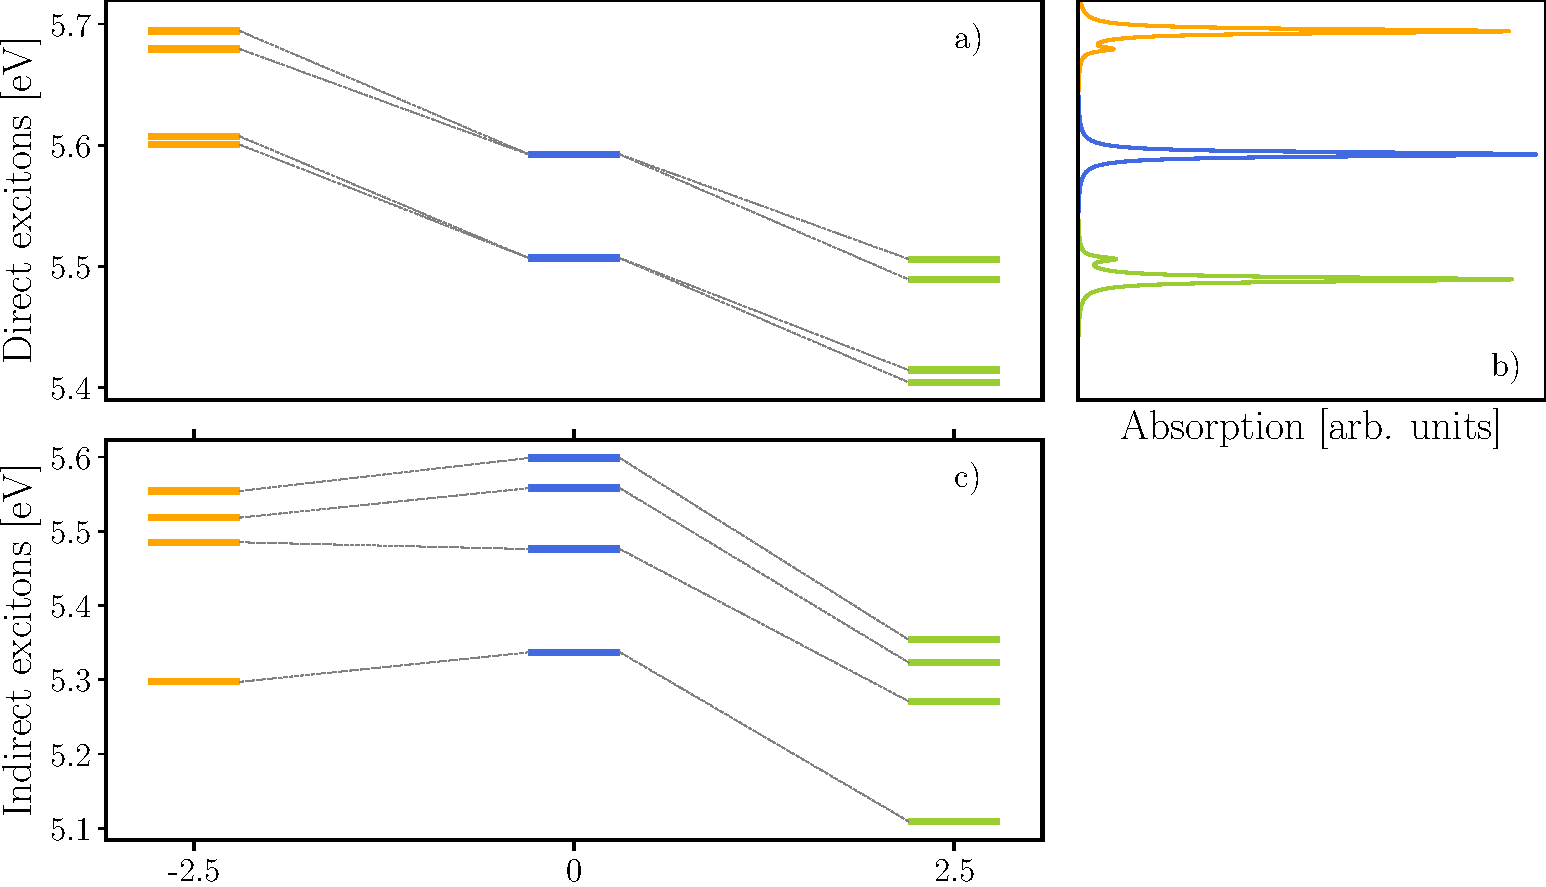
\includegraphics[width=0.8\textwidth]{hBN_exc_abs_vs_strain.pdf}
	\caption{Blue lines are for equilibrium crystal, orange is for compression and green is for stretch. (a) Energies of the lowest 4 excitons at $\Gamma$ (b) Absorption spectra associated with the direct excitons. Both excitons of the bright Davydov pair have a non-zero dipole matrix element and we can distinguish two peaks in the spectra for the strained crystals. (c) Energies of the lowest 4 indirect excitons.}
	\label{fig:exc_abs_vs_strain}
\end{figure}

The associated absorption spectra are displayed in panel (b) of Fig. \ref{fig:exc_abs_vs_strain}. As the inversion symmetry is not broken by uniaxial strain, the lowest two excitons remain dark when strain is applied. For the third and fourth lowest excitons in the strained systems, they are not mixed by the rotational symmetry as it is the case in the pristine crystal. This gives both excitons a non-zero dipole, and we see two peaks appearing in the absorption spectra. \\
The change of peak energy induced by strain is quantified by the strain gauge factor, which is defined as the spectral shift per \% of uniaxial strain. With these calculations, we find a value of $\approx$ 43 meV/\%, which is in the same range as transition metal dichalcogenides as reported in Ref. \cite{carrascoso2021strain}.

The splitting is also visible on the exciton wavefunctions in real space. It is displayed for the lowest two excitons at $\Gamma$, for a stretch of +2.5\%. The splitting is clear, with one of the wavefunctions having its components along the strained B-N bond or the armchair direction, while the other has its components along the zigzag direction.
\begin{figure}[tbp]
	\vspace{0.2cm}
	\setcapindent{2em}
	\centering
	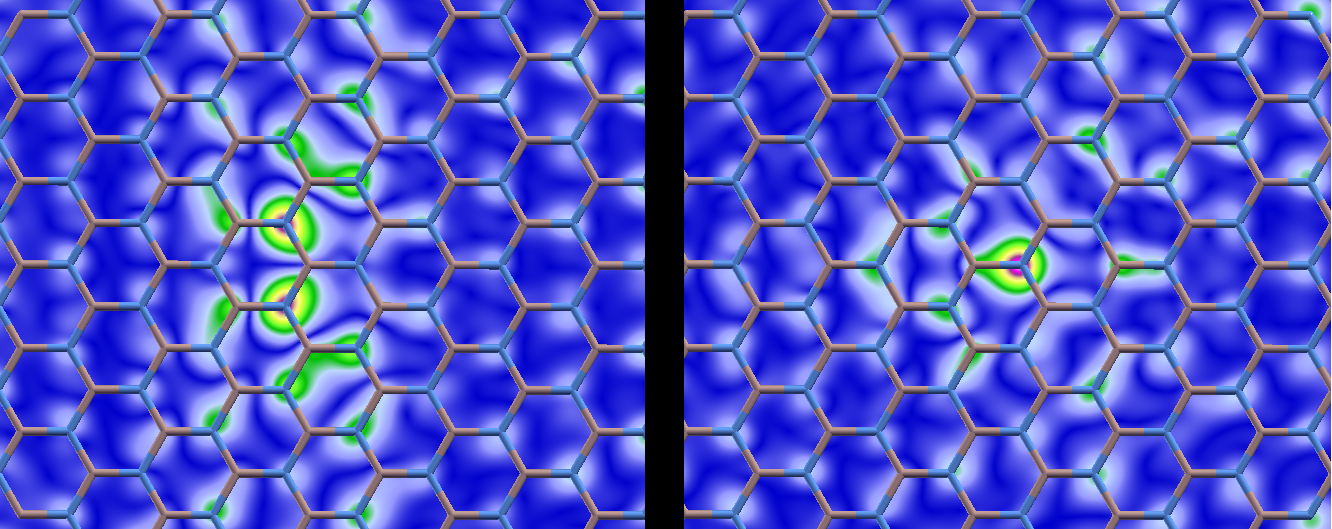
\includegraphics[width=0.8\textwidth]{excitonWF_strain.png}
	\caption{Electron distribution when the hole is fixed near the central Nitrogen atom, that we call exciton wavefunction. Left is the lowest dark exciton at $\Gamma$, right is the second lowest dark exciton at $\Gamma$, taken for a stretch of +2.5\%.}
	\label{fig:excWF_strain}
\end{figure}

We observe the same trend for the lowest-lying excitons with non-zero momentum, which we will call indirect excitons because they are formed by indirect electronic transitions. Their change in energy with strain is reported in Fig. \ref{fig:exc_abs_vs_strain} (c). It follows the same variation as the indirect gap and here again their binding energy is almost invariant with strain. The indirect excitons of hBN play an important role in light emission by luminescence. These changes in energy combined with the change in phonon frequencies will have an impact on the luminescence spectra of the strained crystals. This will be discussed in the next two sections.

%
\section{Exciton-phonon coupling from finite differences}
As presented in the introduction of the thesis, the inclusion of lattice vibrations in our computational framework is necessary to describe accurately the phonon-assisted features in the luminescence spectrum of hBN. In particular the exciton-phonon coupling is the central quantity to take into account. To do so, I present in this section how to calculate the macroscopic dielectric function with a static correction due to lattice vibrations, in a finite-difference scheme. The method can be found in Ref. \cite{paleari2019exciton} and in a slightly different approach in Ref. \cite{cannuccia2019theory}.\\
The key idea is to take the Taylor expansion of the macroscopic dielectric function with respect to atomic displacements. By displacing the atoms around their equilibrium positions along the phonon eigenvectors obtained earlier with \acrshort{DFPT} and calculating the response function with the \acrshort{BSE} in the displaced configurations, we will obtain the coupling between the exciton responsible for the optical response and the phonons. The link between the response function (without the long-range component) and the macroscopic dielectric function is given by Eq. \eqref{eq:eps_macro}. 
The Taylor exp is $\varepsilon (\omega)\approx \varepsilon^{(0)}(\omega) + \varepsilon^{st,(2)}_{\bar{q}}(\omega)$, where the second term is the static correction induced buy the atomic displacements.\cite{zacharias2016one} 
The contribution from exciton $\lambda$ to the response function  writes :
\begin{equation}
	\chi^\lambda_R(\omega) = \frac{|T^\lambda_R|^2}{E^\lambda_R - \omega + i \eta} \label{eq:chi_R_lambda}
\end{equation}
where the subscript R indicates that the quantities are evaluated at clamped ion positions. The infinitesimal $\eta$ is taken independent of $R$ for simplicity. Here we recall that we define the exciton dipole matrix element $T^\lambda = \sum_{cvk} \bar{A}_\lambda^{cvk} d_{cvk}$. The first derivative entering in the Taylor expansion will be :
\begin{equation}
	\frac{\partial \chi^\lambda_R(\omega)}{\partial R}\biggr|_{R=0} = \frac{\partial |T^\lambda_R|}{\partial R}\biggr|_{R=0} \frac{2|T^\lambda_{R=0}|}{E^\lambda_{R=0} - \omega + i\eta} + \frac{\partial \left[ E^\lambda_R - \omega + i\eta \right]^{-1}}{\partial R}\biggr|_{R=0} |T^\lambda_{R=0}|^2.
\end{equation}
This expression has a term linear in the exciton dipole and a term at the second power, both taken at clamped ion positions. It means that for dark excitons, the first derivative in the Taylor expansion will be zero. Excitons belonging in this category are labelled $\lambda'$, and we have $\frac{\partial \chi^{\lambda'}_R(\omega)}{\partial R}\bigr|_{R=0} = 0$.
In \acrshort{hBN}, the excitons involved in luminescence are the ones which low at the lowest energies in the dispersion, at finite momentum. Because of momentum conservation, these ones cannot recombine and emit light which has almost zero momentum, hence they are dark at clamped ion positions. Phonons are needed to transfer momentum and assist their recombination. \\ 
Similar arguments hold for the second derivative in the Taylor expansion
and the only non-vanishing term that remains is :
\begin{equation}
	\frac{\partial^2 \chi^{\lambda'}_R(\omega)}{\partial R^2} = \frac{\partial^2 |T^{\lambda'}_R|^2}{\partial R^2}\biggr|_{R=0} \left[ E^{\lambda'}_{R=0} - \omega + i\eta \right]^{-1} \label{eq:chi_fdd}
\end{equation}
This equation shows that it is equivalent to compute the finite-difference derivative of the full response function or only of the exciton dipoles. This is verified numerically in Ref. \cite{paleari2019exciton}. \\
This above second derivative is evaluated numerically with the finite difference formula :
\begin{equation}
	\frac{\partial^2 \chi^{\lambda'}_R(\omega)}{\partial R^2} \approx \frac{\chi(\Delta\RR;\omega) - 2 \chi_0(\omega) + \chi(-\Delta\RR;\omega)}{\Delta\RR^2}
\end{equation}
In our case, the displacements write $R \to R_{\mu\bar{q}}$ and are along the eigenvector of a particular phonon mode $\mu$ taken at the momentum $\bar{q}$ where the exciton dispersion reaches its minimum. The displacement magnitude are given by Eq. \eqref{eq:normal_displacements} taken for $t=0$ :
\begin{equation}
	u^{\mu\bar{q}}_{Ls\alpha}(t=0) = \frac{c}{\sqrt{M_s}}\Re\left\{ e^{i\bar{\qq}\cdot\boldsymbol{\tau}_L} \xi^{\mu\bar{q}}_{s\alpha} \right\}
\end{equation}
The $c$ parameter is a scaling factor which needs to be converged. Indeed for the finite difference derivative, we want to keep the displacements as small as possible. However if they are too small, their effect will be indistinguishable from numerical noise, but if they are too large, effects beyond the second-order derivatives will start to appear. For this work, we converged the displacements to a value of $|\Delta \RR| = 0.05 \AA$.
To accommodate the periodicity of the phonon at $\bar{q}$, we construct supercells. The supercell with the minimal size is non-diagonal,\cite{lloyd2015lattice} and we build them using the \texttt{yambopy} Python tool.\cite{Sangalli_2019}\\
From Ref. \cite{zacharias2020theory}, the second-order correction to the full dielectric due to the transitions assisted by a single phonon of momentum $\bar{q}$ is :
\begin{equation}
	\varepsilon^{st,(2)}_{\bar{q}} (\omega) = \frac{1}{2} \sum_\mu \left[ \sum_i^{N_{\bar{q}}} \frac{1}{2} \sum_j^2 \frac{\partial^2 \varepsilon^{(0)}_j(\omega)}{\partial R^2_{\mu\bar{q}}} \biggr|_{eq} \right] \sigma^2_{\mu\bar{q}} \label{eq:eps_Taylor_2nd}
\end{equation}
where $j$ is the polarization direction of the incoming light. We average over two orthogonal in-plane directions. The index $i$ runs over the equivalent $\bar{q}$ points in the \acrshort{BZ} where the exciton energies are minimal. For a perfect hBN crystal, $N_{\bar{q}} = 6$ but in our case, $N_{\bar{q}} = 4$. The last factor $\sigma^2_{\mu\bar{q}}$ is the thermal average of the squared displacement of the a quantum harmonic oscillator, given by :
\begin{equation}
	\sigma^2_{\mu\bar{q}}(T) = l^2_{\mu\bar{q}} (2n_{\mu\bar{q}}(T) + 1).
\end{equation}
$n_{\mu\bar{q}}(T)$ is the Bose-Einstein occupation function, and $l^2_{\mu\bar{q}} = 1/(2M_{\mu\bar{q}}\Omega_{\mu\bar{q}})$ is the zero-temperature squared displacement (from now on we refer to phonon frequencies with capital Omega). In our case the reference mass is $M_{\mu\bar{q}} = \sum^{N_{ions}}_s M_s |\xi_s^{\mu\bar{q}}|^2$.\\
Finally the imaginary part of the dielectric function follows from Eqs. \eqref{eq:chi_fdd},\eqref{eq:chi_R_lambda} and \eqref{eq:eps_macro} : 
\begin{equation}
	\Im\frac{\partial^2 \varepsilon^{(0)}(\omega)}{\partial R^2_{\mu\bar{q}}}\biggr|_{eq} = \frac{8\pi}{N_k V} \sum_{\lambda'} \frac{\partial^2 |T^{\lambda'}|^2}{\partial R^2_{\mu\bar{q}}}\biggr|_{eq} \Im\left\{ \frac{1}{\omega - E^{\lambda'} + i\eta} \right\}.
\end{equation}
At this point we can reintroduce the dependence on the phonon frequency coming from the energy conservation in perturbation theory, which was neglected above (more details can be found in Ref. \cite{paleari2019first}). Two terms appear, one coming from the process of phonon emission which is proportional to $1 + n_{\mu\bar{q}}$ and one from phonon absorption proportional to $n_{\mu\bar{q}}$. At low temperature, $1 \gg n_{\mu\bar{q}}$ which means that absorbing a phonon is much less likely than emitting one. We have the transformation :
\begin{equation}
	\frac{2n_{\mu\bar{q}} + 1}{\omega - E^{\lambda'} + i\eta} \to \frac{n_{\mu\bar{q}} + 1}{\omega - E^{\lambda'} - \Omega_{\mu\bar{q}} + i\eta} + \frac{n_{\mu\bar{q}}}{\omega - E^{\lambda'} + \Omega_{\mu\bar{q}} + i\eta}
\end{equation}
Finally, similarly to Ref \cite{paleari2019exciton}, we rename the numerator between square brackets in Eq. \eqref{eq:eps_Taylor_2nd} as $|t^{\text{static}}_{\mu\bar{q}\lambda'}|^2$. It represents the static formation probability of an exciton $\lambda'$ mediated by a phonon mode $\mu$ with momentum $\bar{q}$ and frequency $\Omega_{\mu\bar{q}}$. We can call this quantity \textit{exciton-phonon coupling} matrix element in the sense of optical absorption and exciton creation. This is to be compared with the exciton-phonon matrix elements obtained \textit{ab initio} in Chapter 3.\\
The final expression writes :
\begin{equation}
	\varepsilon^{(2)}_{\bar{q}2}(\omega) = \sum_{\lambda\lambda'} |t^{\text{static}}_{\mu\bar{q}\lambda'}|^2 l^2_{\mu\bar{q}} \left[ n_{\mu\bar{q}} + 1/2 \mp 1/2 \right] \delta(\omega - E^{\lambda'} \pm \Omega_{\mu\bar{q}}). \label{eq:eps2_fdd}
\end{equation}
The upper (lower) sign refers to the process of phonon absorption (emission). One thing to note here is that we neglect the variation of the exciton energies induced by the coupling with phonon. This is justified for hBN because the exciton energies are large enough compared to this renormalization, and moreover we know that the $GW$ approximation underestimates the fundamental gap, so the energies we will obtain at the end of the process will not be accurate anyways. Instead, we focus on obtaining spectra that reproduce the shape of phonon-assisted replicas.

%
\section{Luminescence results}
We used the expression of the dielectric function in Eq. \eqref{eq:eps2_fdd} and plugged it in the van Roosbroeck--Shockley relation from Eq. \eqref{eq:vRS_PL_ind}. The full expression writes :
\begin{multline}
	R^{sp}(\omega)= \sum_{\mu,{\bar{q}}} \frac{\omega(\omega + 2\Omega_{\mu \bar{q}})^2}{\pi^2 c^3 } n_1(\omega) \sum_S \frac{\partial^2 |T^{\lambda'}|^2 }{\partial R_{\mu\bar{q}}^2}\biggr|_{\text{eq}} \\ \times	\Im \left\{\frac{1}{\omega-(E^{\lambda'}-\Omega_{\mu \bar{q}})+i\eta}\right\} n_B(E^{\lambda'}_{\bar{q}},T_{exc})
\end{multline}
where $n_B(E^{\lambda'}_{\bar{q}},T_{exc}) = e^{-(E^{\lambda'}-E^{min})/k_BT_{exc}}$ is the Boltzmann occupation for excitons where the energy difference is taken with the minimal exciton energy over the whole Brillouin Zone $E^{min}$. It means that the lowest valleys in the exciton dispersion will be populated by relaxed excitons, while the higher states will have exponentially decaying populations. For instance, the direct exciton has an energy too large to even be visible in the spectrum.
As discussed above, we simulate a crystal at low temperature, which we set at 10K in agreement with the experimental measurements. Hence we approximated $1 + n_{\mu\bar{q}} \approx 1$, and we neglect the phonon absorption processes, which would give higher energy peaks that would be suppressed by the Boltzmann function anyway. The excitonic temperature $T_{exc}$ is higher than the lattice temperature because we consider a steady-state process in which the excitons do not thermalize, since they are constantly pumped by the laser. We obtained the value by fitting the experimental data of Ref. \cite{cassabois2016hexagonal} which gave us the value of $T_{exc} = 24 K$ for a lattice temperature of $T_L = 10 K$. The effect of temperature is also taken into account in the broadening parameter of the peaks with the Lorentzian model : $\eta = \Gamma_0 + aT + bB(T)$ where the values of the parameters can be found in Refs. \cite{paleari2019exciton,vuong2017exciton}. Another approximation we made is to compute the dipoles at the displaced configurations with the statically screened interaction from the equilibrium configurations : 
\begin{equation}
	\frac{\partial^2 |T^{\lambda'} (W, L )|^2 }{\partial R_{\mu \bar{q}}^2} \simeq \frac{\partial^2 |T^{\lambda'} (W(R=R_{eq}), L) |^2 }{\partial R_{\mu \bar{q}}^2}.
\end{equation}
It has been shown previously that this has negligible effects for the calculation of electron-phonon matrix elements,\cite{faber2015exploring} and we verified that our results are not modified by this approximation. 

Now comes the discussion about the choice of $\bar{q}$. For the pristine hBN crystal, the indirect electronic gap is between two points close to the \KK~point and the \MM~point. The usual approximation is to consider that the gap lies on the \KK~point, and that the momentum that connects the two points is $\qq = (\tfrac{1}{3}, -\tfrac{1}{6}, 0)$ and that the minimum of the exciton dispersion is also at this momentum. This simplifies the construction of the supercells needed to accommodate the phonon modes at this $\qq$-vector. In our case, because of the symmetry breaking in the electronic dispersion, there are several indirect gaps which have a very similar energy, especially for low values of strain. This could lead to a broadening of the peaks in the luminescence spectra. In order to verify this hypothesis, we constructed the supercells which accommodate all the vectors corresponding to the transitions $\bf M - \bf K$,  $\bf M - \bf {K'}$,  $\bf {M'} - \bf K$ , $\bf {M'}  - \bf { K'}$. Then we performed a \acrshort{BSE} calculation for all these non-diagonal supercells containing 24 displaced atoms and summed the dipoles. Because of the displacement of atoms, some symmetries are broken and the dark excitons which are folded at $\Gamma$ acquire a finite dipole, hence contributing to the luminescence spectra.\\

The resulting spectra for various values of strained are displayed in Fig. \ref{fig:Lum_vs_strain}.
\begin{figure}[tbp]
	\vspace{0.2cm}
	\setcapindent{2em}
	\centering
	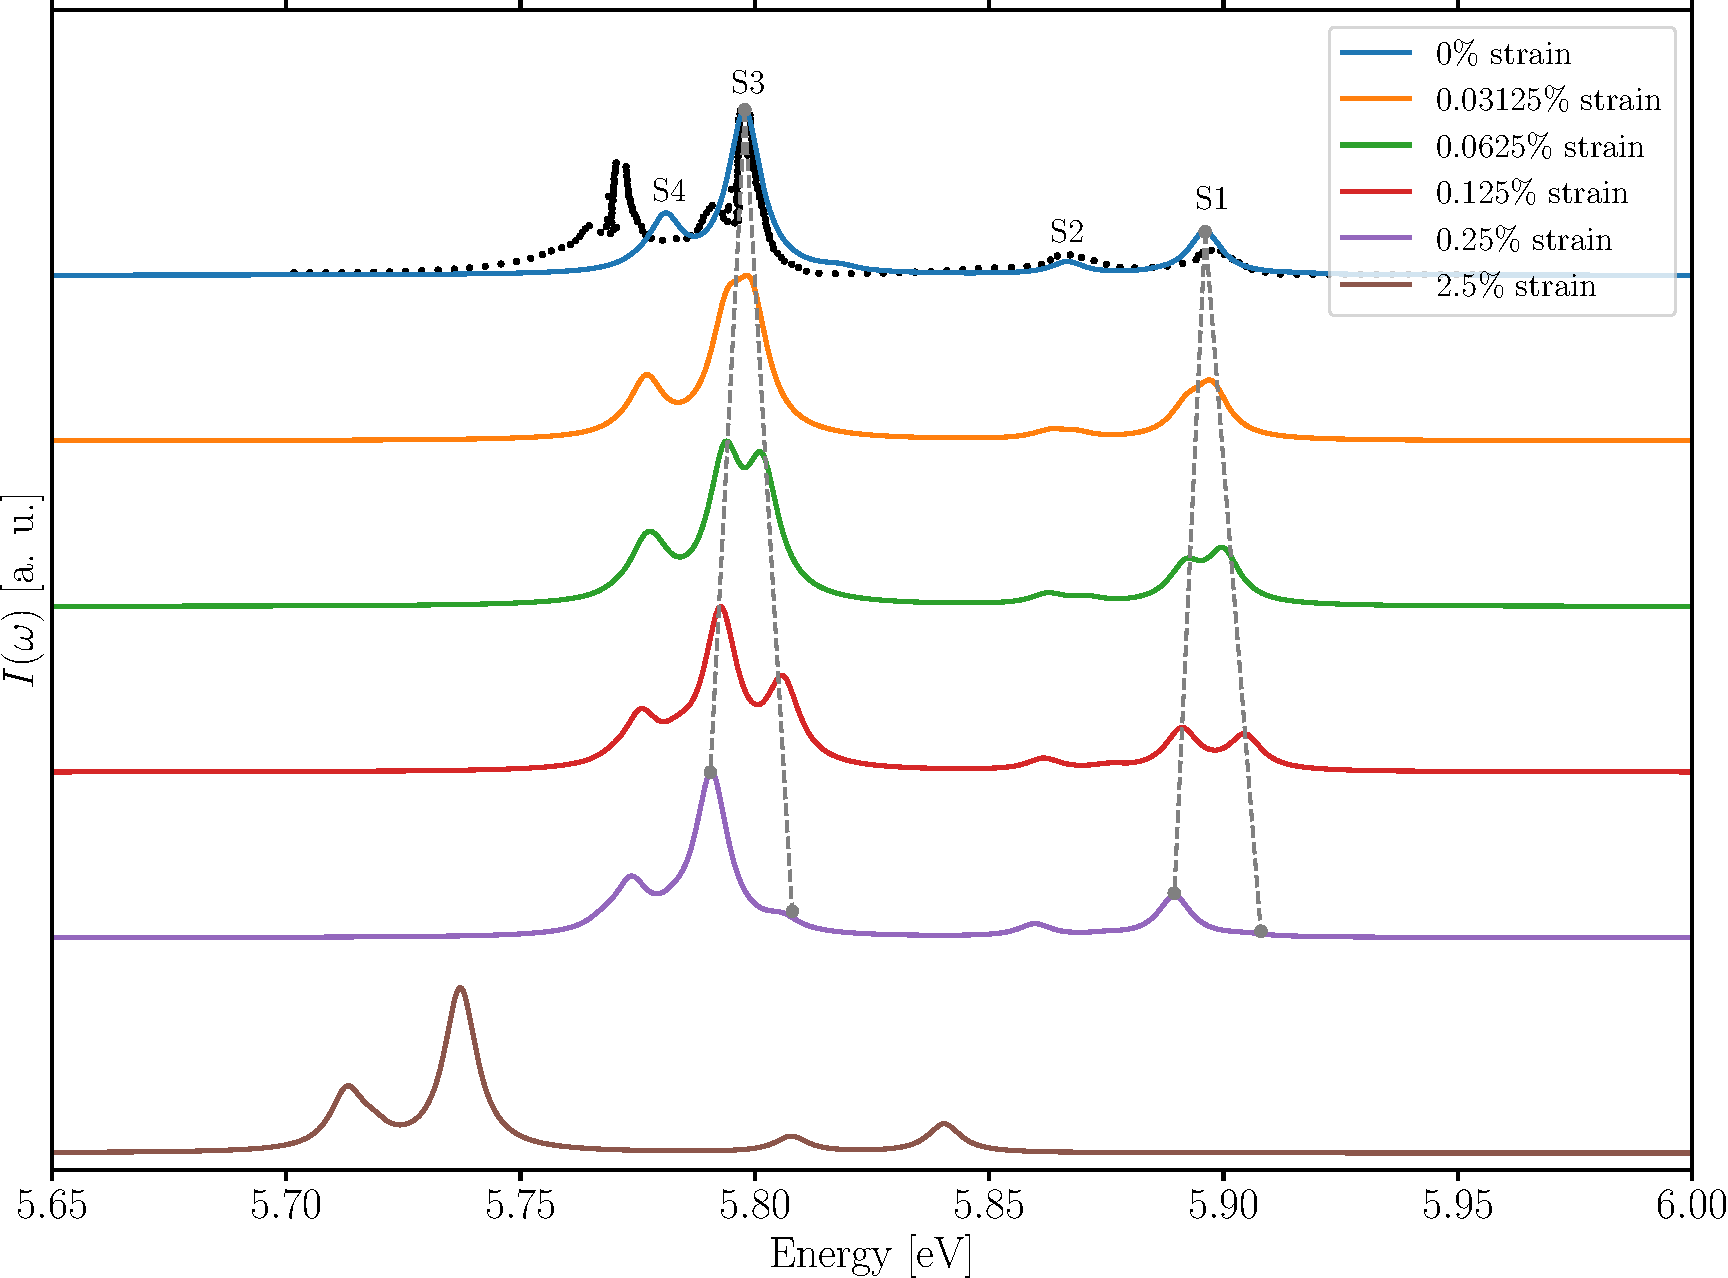
\includegraphics[width=0.9\textwidth]{Lum_vs_strain.pdf}
	\caption{Luminescence spectra as a function of strain, for selected value of compressive strain. Plots are shifted vertically for clarity. On the top plot, experimental data is represented by the black dots from Ref. \cite{schue2019bright}. The spectra have been shifted to match the position of the indirect exciton at equilibrium, and compensate the numerical error of the $GW$ approximation.\cite{artus2021ellipsometry} Dashed lines are a guide for the eye.}
	\label{fig:Lum_vs_strain}
\end{figure}
First, we can see on the top plot that the equilibrium luminescence spectrum is quite well reproduced compared to experiment. At low values of strain, the excitons originating from the different $\bf{ M^{(')}} - \bf{ K^{(')}}$ transitions have a very close energy and therefore all of them contribute to the luminescence spectra as they are not suppressed by the Boltzmann function. These excitons scatter with phonons who also have their frequencies modified. These combined effects create a splitting of the peaks which increases with strain. There is also a slight increase in the intensty of the S1 and S2 peaks, coming from scattering with LA and TA modes. At equilibrium, we found that the S3/S1 intensity ratio is $\approx 3.7$ and it decreases down to $\approx 2.7$ with strain. This result is in line with those of Léonard Schué in Ref. \cite{schue2017proprietes}, however they found a ratio going down to $\approx 1$ in their compressed samples.\\ The discrepancy could be explained by the lack of the fine sampling of the exciton and phonon dispersions. Indeed with a larger density of states to scatter, the intensity of some peaks could be increased even more. The differences could also come from experimental factors not accounted for in our simulation methods, such as surface effects or non-uniform strain field.\\
Finally, for larger values of strain, the exciton energies split so much that the peaks coming from the higher one are suppressed by the Boltzmann function in the van Roosbroeck--Shockley relation. The spectrum thus acquires the same shape as the equilibrium one but translated to lower energies due to the closure of the indirect gap, and the change in the phonon frequencies. Note that the $2.5\%$ value of strain is extreme and is probably out of reach in the experimental conditions we try to reproduce. The results are similar for the tensile strain.

%
\section*{Conclusion of the chapter}
In this chapter, I presented our results about the electronic, phononic and optical properties of bulk hBN under uniaxial strain, both tensile and compressive., along the armchair direction. We observed a splitting of the exciton at $\Gamma$ due to the breaking
of the threefold rotational symmetry. This splitting could be measured in reflectivity experiments.\cite{elias2021flat} We also found that the direct excitons energies vary linearly with the applied strain, while the indirect exciton energies decrease both with compression and stretch. We were also able to evaluate the strain gauge factor, which was found to be similar to that of transition metal dichalcogenides.
I presented a method to include the exciton-phonon coupling in the response function and hence in the optical spectra of the strained crystals. It is based on a finite-difference derivative approach and is well-suited for materials with a indirect and deep exciton dispersion exciton minimum. The coupling of excitons and phonons is calculated only for a few momenta in the Brillouin Zone. Since this method requires the use of supercells, it is particularly adapted to the study of defects such as in Ref. \cite{libbi2022phonon}. We employed the method to compute the phonon-assisted luminescence spectrum and how it changes with strain. We found that at low strain,additional peaks appear in the spectra due to the breaking of the degeneracy between the different \KK~ and \MM~ points in the Brillouin Zone. These additional peaks decrease the intensity ratio between the acoustic- and the optical-phonon assisted transitions, in agreement with recent measurements. For large compressive strain we found that only one valley contributes to the luminescence, and the spectra return to a shape similar to the equilibrium one but shifted at lower energies. This prediction could be verified by means of luminescence measurements in highly strained h-BN.\cite{blundo2022vibrational}

	\chapter{Ab initio exciton-phonon coupling}
\chaptertoc{}

\section{Introduction}
Mainly on monolayer, the three experiments
mention also the cathodoluminescence paper in which we see only the direct peak
say we did a benchmark on hBN
talk about the bBN and the reason we chose it : direct and indirect gaps are close in energy so we might see direct peak and phonon satellites. Indeed it was see experimentally so it is a good candidate for our method.

\section{monolayer exciton dispersion}
fitting of the dispersion, Lbar vs Lfull
the nearly-free electron states at Gamma

\section{Theory of the ab initio exciton-phonon coupling}
The derivation in MBPT is carried out in Pierluigi Cuddazzo's paper in 2020 and with extensive details in Fulvio's thesis. Here we follow a different approach, similar to Chen's derivation. I should mention the fact that they compute the exc-ph matrix elements like us, but the luminescence is different.\\
For simplicity, drop $\QQ$.
exciton creation and annihilation operators\\

We consider a system with displacements from the equilibrium positions $\boldsymbol{u}_{Ls}$ ($L$ labels the unit cell and $s$ the atom). Taylor expansion of the Kohn-Sham potential around the equilibrium positions :
\begin{equation}
    V^{KS}(\left\{ \uu_{Ls} \right\}) = V_0^{KS} + \sum_{Ls\alpha} \frac{\partial V^{KS}}{\partial \uu_{Ls\alpha}} \uu_{Ls\alpha} + \mathcal{O}(\left\{ \uu_{Ls} \right\}^2)
\end{equation}
The electronic wave functions and eigenvalues of the perturbed system depend on the atomic displacements $\left\{ \uu_{Ls} \right\}$. To obtain their change in the perturbed system, we apply first-order perturbation theory by keeping terms linear in $\left\{ \uu_{Ls} \right\}$. To first order, the correction to the eigenvalues vanishes while the correction to the Kohn-Sham wave functions $\psi_i$, (solutions of Eq. \eqref{eq:KS_eqs}) can be written as : 
\begin{equation}
    \delta\ket{\psi_i} = \sum_{j\neq i} \frac{\bra{\psi_j} \Delta V \ket{\psi_i}}{\epsilon_i - \epsilon_j} \ket{\psi_j}, \qquad \text{with} \ \ \Delta V = \sum_{Ls\alpha}\frac{\partial V^{KS}}{\partial \uu_{Ls}}\cdot \uu_{Ls}
\end{equation}
In the following, we use the tilde for quantities of the perturbed system and write the perturbed wave function as :
\begin{equation}
    \ket{\tilde{\psi}_i} = \ket{\psi_i} + \delta\ket{\psi_i} = \ket{\psi_i} + \sum_{j \neq i} \Delta_{ij} \ket{\psi_j}
\end{equation}
with
\begin{equation}
    \Delta_{ij} \equiv \frac{\bra{\psi_j} \Delta V \ket{\psi_i}}{\epsilon_i - \epsilon_j}
\end{equation}

We start by defining an unpertubed Bethe-Salpeter Hamiltonian $H \equiv H(\{\boldsymbol{u}_{Ls} \}=0)$ and a perturbed BSE Hamiltonian $\Tilde{H} \equiv H(\{\boldsymbol{u}_{Ls} \})$. We will use first order perturbation theory to obtain the exciton-phonon interaction. The BSE Hamiltonian writes :
\begin{equation}
    H_{vc,v'c'} = \bra{vc} H \ket{v'c'} = ( \epsilon_c - \epsilon_v ) \delta_{vv'}\delta_{cc'} + K_{vc,v'c'}
    \label{eq:BSE_H}
\end{equation}
where $c,v$ are for conduction and valence band, respectively. The perturbed Hamiltonian one is :
\begin{equation}
    \Tilde{H}_{\Tilde{v}\Tilde{c},\Tilde{v}'\Tilde{c}'}  = \bra{\Tilde{v}\Tilde{c}} H \ket{\Tilde{v}'\Tilde{c}'}  = ( \Tilde{\epsilon}_c - \Tilde{\epsilon}_v ) \delta_{\Tilde{v}\Tilde{v}'}\delta_{\Tilde{c}\Tilde{c}'} + K_{\Tilde{v}\Tilde{c},\Tilde{v}'\Tilde{c}'}
\end{equation}
The Bethe-Salpeter kernel is defined as :
\begin{equation}
    K_{vc,v'c'} = \bra{vc} K \ket{v'c'} = \int d1 d2 d3 d4 \psi_v(2) \psi_c^*(1) K(1234) \psi^*_{v'}(3)\psi_{c'}(4)
\end{equation}
where
\begin{equation}
    K(1234) = -i\delta(1,2)\delta(3,4)\ v(1,4) + i \delta(1,4)\delta(2,3)\ W(1,2)
\end{equation}
with $v$ being the bare Coulomb potential and $W$ the screened Coulomb interaction. In the fashion of Many-Body theory, space, time and spin variables are grouped like so : $1 = (\boldsymbol{r_1},t_1,\sigma_1)$. $\Tilde{K}_{\Tilde{v}\Tilde{c},\Tilde{v}'\Tilde{c}'}$ is the 
\begin{equation}
    \Tilde{K}_{\Tilde{v}\Tilde{c},\Tilde{v}'\Tilde{c}'} = \bra{\Tilde{v}\Tilde{c}} \Tilde{K} \ket{\Tilde{v}'\Tilde{c}'} 
\end{equation}
Solving the BSE Hamiltonian in \eqref{eq:BSE_H} gives the exciton wave functions $\ket{S_n}$ and energies $E^{S_n}$ :
\begin{align}
    \sum_{v',c'} H_{vc,v'c'} A^{S_n}_{v'c'} &= E^{S_n} A^{S_n}_{vc} \\
    \ket{S_n} = \sum_{vc}& A_{vc}^{S_n}\ket{vc}
\end{align}
To derive the exciton-phonon interaction, we project the perturbed BSE Hamiltonian onto the unperturbed basis set and keep only the terms to first-order in the phonon perturbation. By such a process, the terms that will arise and be different from the unperturbed BSE Hamiltonian will define the exciton-phonon interaction. One can show that to first order, the perturbed and unperturbed electronic energies coincide, so we will use $\Tilde{\epsilon}_i = \epsilon_i$. The perturbed Hamiltonian in the unperturbed basis is :
\begin{align*}
    \Tilde{H}_{nm} = \bra{S_m} \Tilde{H} \ket{S_n} &= \sum_{\Tilde{v}\Tilde{c},\Tilde{v}'\Tilde{c}'}  \bra{S_m}\ket{\Tilde{v}\Tilde{c}}\bra{\Tilde{v}\Tilde{c}} \Tilde{H} \ket{\Tilde{v}'\Tilde{c}'}\bra{\Tilde{v}'\Tilde{c}'}\ket{S_n} \\
    &= \sum_{vc,v'c'}\sum_{\Tilde{v}\Tilde{c},\Tilde{v}'\Tilde{c}'} \bra{S_m}\ket{vc}\bra{vc}\ket{\Tilde{v}\Tilde{c}}\bra{\Tilde{v}\Tilde{c}} \Tilde{H} \ket{\Tilde{v}'\Tilde{c}'}\bra{\Tilde{v}'\Tilde{c}'}\ket{v'c'}\bra{v'c'}\ket{S_n}
\end{align*}
where we used the completeness relations of both basis sets, $\sum_{vc}\ket{vc}\bra{vc} = 1$ and $\sum_{\Tilde{v},\Tilde{c}} \ket{\Tilde{v}\Tilde{c}}\bra{\Tilde{v}\Tilde{c}} = 1$. By definition of the BSE wave functions $\bra{v'c'}\ket{S_n} = A^{S_n}_{v'c'}$, then we can write the above equation as :
\begin{equation}
    \Tilde{H}_{nm} = \bra{S_m} \Tilde{H} \ket{S_n} = \sum_{vc,v'c'} A{^S_m *}_{vc} A^{S_n}_{v'c'} \times \left[ \sum_{\Tilde{v}\Tilde{c},\Tilde{v}'\Tilde{c}'} \bra{vc}\ket{\Tilde{v}\Tilde{c}}  \bra{\Tilde{v}\Tilde{c}} \Tilde{H} \ket{\Tilde{v}'\Tilde{c}'} \bra{\Tilde{v}'\Tilde{c}'}\ket{v'c'} \right]
    \label{eq:exc_ham}
\end{equation}
The term inside the square brackets can be separated into to terms :
\begin{align*}
    &\sum_{\Tilde{v}\Tilde{c},\Tilde{v}'\Tilde{c}'} \bra{vc}\ket{\Tilde{v}\Tilde{c}}  \bra{\Tilde{v}\Tilde{c}} \Tilde{H} \ket{\Tilde{v}'\Tilde{c}'} \bra{\Tilde{v}'\Tilde{c}'}\ket{v'c'} =  \sum_{\Tilde{v}\Tilde{c},\Tilde{v}'\Tilde{c}'} \bra{vc}\ket{\Tilde{v}\Tilde{c}}  \left[ (\Tilde{\epsilon}_{\Tilde{c}} - \Tilde{\epsilon}_{\Tilde{v}}) \delta_{\Tilde{v}\Tilde{v}'}\delta_{\Tilde{c}\Tilde{c}'} + \Tilde{K}_{\Tilde{v}\Tilde{c},\Tilde{v}'\Tilde{c}'} \right] \bra{\Tilde{v}'\Tilde{c}'}\ket{v'c'} \\
    &= \sum_{\Tilde{v}\Tilde{c}} \bra{vc}\ket{\Tilde{v}\Tilde{c}} (\epsilon_{\Tilde{c}} - \epsilon_{\Tilde{v}}) \bra{\Tilde{v}\Tilde{c}}\ket{v'c'} + \sum_{\Tilde{v}\Tilde{c},\Tilde{v}'\Tilde{c}'} \bra{vc}\ket{\Tilde{v}\Tilde{c}} \Tilde{K}_{\Tilde{v}\Tilde{c},\Tilde{v}'\Tilde{c}'} \bra{\Tilde{v}'\Tilde{c}'}\ket{v'c'}
\end{align*}
We make the choice to approximate the perturbed kernel with the unperturbed one, $\Tilde{K}_{\Tilde{v}\Tilde{c},\Tilde{v}'\Tilde{c}'} \approx \bra{\Tilde{v}\Tilde{c}}K\ket{\Tilde{v}'\Tilde{c}'}$, that is to say the effect of the atomic displacements on the bare and screened Coulomb interactions can be neglected and $W \approx \Tilde{W}$. With this approximation we have :
\begin{equation}
    \sum_{\Tilde{v}\Tilde{c},\Tilde{v}'\Tilde{c}'} \bra{vc}\ket{\Tilde{v}\Tilde{c}} \Tilde{K}_{\Tilde{v}\Tilde{c},\Tilde{v}'\Tilde{c}'} \bra{\Tilde{v}'\Tilde{c}'}\ket{v'c'} 
    \approx  \sum_{\Tilde{v}\Tilde{c},\Tilde{v}'\Tilde{c}'} \bra{vc}\ket{\Tilde{v}\Tilde{c}} 
    \bra{\Tilde{v}\Tilde{c}} K \ket{\Tilde{v}'\Tilde{c}'}\bra{\Tilde{v}'\Tilde{c}'}\ket{v'c'} = \bra{vc} K \ket{v'c'} = K_{vc,v'c'}
\end{equation}
and thus the term in brackets in Eq. \eqref{eq:exc_ham} becomes 
\begin{equation}
    \sum_{\Tilde{v}\Tilde{c},\Tilde{v}'\Tilde{c}'} \bra{vc}\ket{\Tilde{v}\Tilde{c}}  \bra{\Tilde{v}\Tilde{c}} \Tilde{H} \ket{\Tilde{v}'\Tilde{c}'} \bra{\Tilde{v}'\Tilde{c}'}\ket{v'c'} = \sum_{\Tilde{v}\Tilde{c}} \bra{vc}\ket{\Tilde{v}\Tilde{c}} (\epsilon_{\Tilde{v}} - \epsilon_{\Tilde{c}}) \bra{\Tilde{v}\Tilde{c}}\ket{v'c'} +  K_{vc,v'c'} 
\end{equation}
Next, we use Eq. (pas écrite) to expand $\sum_{\Tilde{v}\tilde{c}} \bra{vc}\ket{\Tilde{v}\Tilde{c}} (\epsilon_{\Tilde{c}} - \epsilon_{\Tilde{v}})\bra{\Tilde{v}\Tilde{c}}\ket{v'c'}$ to order $\mathcal{O}(\Delta)$. We work within the Tamm-Dancoff approximation and keep only the resonant part of the BSE Hamiltonian; as a consequence, only valence-valence and conduction-conduction hole- and electron-phonon are allowed, that is to day $\Delta_{vc} = \Delta_{cv} = 0$. Using Eq. (pas écrite) we get :
\begin{align}
\begin{split}
    \bra{vc}\ket{\tv\tc} &= \bra{v}\ket{\tv}\bra{c}\ket{\tc} = \left(\delta_{v\tv} + \sum_{v''\neq\tv}\Delta_{\tv v''}\delta_{vv''}\right) \left(\delta_{c\tc} + \sum_{c''\neq \tc}\Delta_{\tc c''}\delta_{cc''}\right) \\
    &= \left( \delta_{v\tv}\delta_{c\tc} + \delta_{v\tv} \sum_{c''\neq\tc} \Delta_{\tc c''}\delta_{cc''} + \delta_{c\tc}\sum_{v''\neq \tv} \Delta_{\tv v''} \delta_{vv''} \right) + \mathcal{O}(\Delta^2)
\end{split}
\end{align}
and similarly
\begin{equation}
    \bra{\tv\tc}\ket{v'c'} = \bra{v'}\ket{\tv}^*\bra{c'}\ket{\tc}^* = \left( \delta_{v'\tv}\delta_{c'\tc} + \delta_{v'\tv} \sum_{c''\neq\tc} \Delta^*_{\tc c''}\delta_{c'c''} + \delta_{c'\tc}\sum_{v''\neq \tv} \Delta^*_{\tv v''} \delta_{v'v''}  \right)  + \mathcal{O}(\Delta^2)
\end{equation}
With these expressions, there are five first-order terms in $\sum_{\Tilde{v}\tilde{c}} \bra{vc}\ket{\Tilde{v}\Tilde{c}} (\epsilon_{\Tilde{c}} - \epsilon_{\Tilde{v}})\bra{\Tilde{v}\Tilde{c}}\ket{v'c'}$ that we can simplify using the Kronecker delta :
\begin{align}
    \sum_{\tv\tc} \bra{vc}\ket{\tv\tc} (\epsilon_{\Tilde{c}} - \epsilon_{\Tilde{v}})\bra{\tv\tc}\ket{v'c'} \nonumber \\
    %
        \approx (\epsilon_c - \epsilon_v)\delta_{vv'}\delta_{cc'} &+ \delta_{cc'}\sum_{\tv}(\epsilon_c - \epsilon_{\tv}) \sum_{v''\neq \tv} (\Delta^*_{\tv v''}\delta_{vv''}\delta_{v'\tv} + \Delta_{\tv v''}\delta_{v'v''}\delta_{v\tv}) \nonumber \\
        &+  \delta_{vv'} \sum_{\tc} (\epsilon_{\tc} - \epsilon_v) \sum_{c'' \neq\tc} (\Delta_{\tc c''}\delta_{cc''}\delta_{c'\tc} + \Delta^*_{\tc c''}\delta_{c'c''}\delta_{c\tc}) \nonumber \\
        %
        = (\epsilon_c - \epsilon_v)\delta_{vv'}\delta_{cc'} &+ \delta_{cc'} \left[  \sum_{v''\neq v'} (\epsilon_c - \epsilon_{v'}) \Delta^*_{v'v''}\delta_{v v''} + \sum_{v'' \neq v} (\epsilon_c - \epsilon_v) \Delta_{vv''} \delta_{v'v''} \right] \nonumber \\
        &+  \delta_{vv'} \left[ \sum_{c''\neq c'} (\epsilon_{c'} - \epsilon_v)\Delta_{c' c''}\delta_{cc''} + \sum_{c''\neq c} (\epsilon_c - \epsilon_v) \Delta^*_{cc''}\delta_{c'c''} \right] \nonumber \\
    %
    = (\epsilon_c - \epsilon_v) \delta_{vv'}\delta_{cc'} &+ \delta_{cc'}(\epsilon_{v'} - \epsilon_v) \Delta_{vv'} + \delta_{vv'}(\epsilon_c - \epsilon_{c'}) \Delta^*_{cc'}
\end{align}
where we used $\Delta_{ij} = -\Delta_{ji}^*$ to obtain the last line. Finally, the perturbed Hamiltonian in the excitonic basis in Eq. \eqref{eq:exc_ham} becomes :
\begin{align}
    \tilde{H}_{mn} &= \sum_{vc,v'c'} A^{S_m *}_{vc} A^{S_n}_{v'c'} \times \left\{ \left[ (\epsilon_c - \epsilon_v) \delta_{vv'}\delta_{cc'} + K_{vc,v'c'} \right] + \delta_{cc'} (\epsilon_{v'} - \epsilon_v)\Delta_{vv'} + \delta_{vv'}(\epsilon_c - \epsilon_{c'}) \Delta_{cc'}^*  \right\} \nonumber \\
    &= E^{S_m}\delta_{mn} + \sum_{vc,v'c'} A^{S_m*}_{vc} A^{S_n}_{v'c'} \cdot \left( \delta_{cc'}(\epsilon_{v'} - \epsilon_v) \Delta_{vv'}  + \delta_{vv'} (\epsilon_c - \epsilon_{c'}) \Delta^*_{cc'} \right) \label{eq:perturb_H_exc}
\end{align}
where we use the fact that the unperturbed Hamiltonian is diagonalized by the Tamm-Dancoff exciton eigenvectors :
\begin{equation}
    E^{S_m}\delta_{mn} = \sum_{vc,v'c'} A^{S_m*}_{vc} A^{S_n}_{v'c'} \times \left( (\epsilon_c - \epsilon_v)\delta_{vv'}\delta_{cc'}+ K_{vc,v'c'} \right).
\end{equation}
Therefore, the first term in the second line of Eq. \eqref{eq:perturb_H_exc} is the unperturbed Hamiltonian, while the second term is the exciton-phonon interaction,
\begin{equation}
    \tilde{H}_{\text{exc-ph}} = \sum_{vc,v'c'} A^{S_m*}_{vc} A^{S_n}_{v'c'} \cdot \left( \delta_{cc'}(\epsilon_{v'} - \epsilon_v) \Delta_{vv'}  + \delta_{vv'} (\epsilon_c - \epsilon_{c'}) \Delta^*_{cc'} \right). \label{eq:H_exc-ph}
\end{equation}
To obtain the final result, we reintroduce the momemtum dependence and the Bloch states :
\begin{equation}
    \ket{\phi_i} \to \ket{\phi_{n\kk}}
\end{equation}
and the transition basis set for an exciton with center of mass momentum $\QQ$ is $\ket{vc} = \ket{v\kk_v,c\kk_c} = \ket{v\kk_v,c\kk_v + \QQ}$. We write the change in potential due to atomic displacements using normal coordinates :
\begin{equation}
    \Delta V = \sum_{\mu \qq} \sqrt{\frac{1}{2\Omega_{\mu\qq}}} \Delta_{\mu\qq} V^{KS}(\hat{b}_{\mu\qq} + \hat{b}^\dagger_{\mu-\qq})  
\end{equation}
Then the $\Delta_{ij}$ describing the transition from $i$-th to $j$-th state becomes :
\begin{equation}
    \Delta_{n\kk n'\kk'} = \frac{\bra{n'\kk'} \Delta V \ket{n\kk}}{\epsilon_{n\kk} - \epsilon_{n'\kk'}} = \sum_{\mu\qq} \frac{g_{nn'v}(\kk,\qq) \delta(\kk'-\kk-\qq)}{\epsilon_{n\kk} - \epsilon_{n'\kk'}} (\hat{b}_{\mu\qq} + \hat{b}^\dagger_{\mu-\qq})
\end{equation}
where $g_{nn'\mu}(\kk,\qq) = (1/2\Omega_{\mu\qq})^{1/2} \bra{n'\kk'} \Delta_{\mu\qq} V^{KS} \ket{n\kk}$ is the usual electron-phonon matrix element \textcolor{red}{check if it corresponds to the expression I gave in chapt1}, namely the probability amplitude for an electron in band $n$ with crystal momentum $\kk$ to transition to a final state in band $n'$ and momentum $\kk' = \kk+\qq$ by absorbing or emitting a phonon with mode index $\mu$ and wave vector $\qq$.

By introducing exciton creation and annihilation operators, $\hat{a}^\dagger_{S_n(\QQ)}$ and $\hat{a}_{S_n(\QQ)}$, we rewrite the exciton-phonon interaction from Eq. \eqref{eq:H_exc-ph} as :
\begin{equation}
    \tilde{H}_{\text{exc-ph}} = \sum_{mn\mu, \QQ\qq} \mathcal{G}_{mn\mu}(\QQ,\qq) \hat{a}^\dagger_{S_n(\QQ+\qq)} \hat{a}_{S_n(\QQ)} (\hat{b}_{\mu\qq} + \hat{b}^\dagger_{\mu-\qq}).
\end{equation}
where we defined the exciton-phonon matrix elements as :
\begin{multline}
    \mathcal{G}_{nm\mu}(\QQ,\qq) = \sum_{\substack{vcv'c'\\ \kk_v \kk_c \kk'_{v'} \kk'_{c'}}} A^{S_m(\QQ+\qq)*}_{v\kk_v,c\kk_c} A^{S_n(\QQ)}_{v'\kk'_{v'},c'\kk'_{c'}} \left[ \delta_{vv'} g_{c'c\mu}(\kk'_{c'},\qq) \delta(\kk_c - \kk'_{c'} - \qq) \right. \\
    \left. - \delta_{cc'}g_{vv'\mu}(\kk_v,\qq) \delta(\kk'_{v'} - \kk_v -\qq) \right]. \label{eq:Gkkp}
\end{multline}
Let us make momentum conservation explicit to obtain the final expression. The exciton-phonon coupling constant $\mathcal{G}_{mn\mu}(\QQ,\qq)$ is the probability amplitude for scattering from an exciton with band index $n$ with center-of-mass momentum $\QQ$ to an exciton with band index $m$ and center-of-mass momentum $\QQ+\qq$. Since $A^{S_n(\QQ)}_{v\kk_{v},c\kk_{c}} \neq 0$ only for $\kk_c - \kk_v = \QQ$ \textcolor{red}{(why ?)}, in Eq. \eqref{eq:Gkkp} we can impose three constraints : $\kk_c - \kk_v = \QQ$, $\kk'_c - \kk'_v =\QQ + \qq$ and $\kk'_c - \kk_c = \qq$ (or $\kk'_v - \kk_v = \qq$). As a consequence, we drop three $\kk$-point \acrshort{BZ} summations and the final result for the exciton-phonon matrix element for a given exciton momentum $\QQ$ and phonon momentum $\qq$ is :
\begin{multline}
    \mathcal{G}_{nm\mu}(\QQ,\qq) = \sum_{\kk} \left[ \sum_{vcc'} A^{S_m(\QQ+\qq)*}_{v\kk,c(\kk+\QQ+\qq)} A^{S_n(\QQ)}_{v\kk,c'(\kk+\QQ)}g_{c'cv}(\kk+\QQ,\qq) \right.\\
     \left. - \sum_{cvv'} A^{S_m(\QQ+\qq)*}_{v(\kk-\qq),c(\kk+\QQ)} A^{S_n(\QQ)}_{v'\kk,c(\kk+\QQ)} g_{vv'\mu}(\kk-\qq,\qq) \right].
\end{multline}

\section{PL benchmark on hBN and results for mBN}
better than Chen but intensity reversed for LO/TO. Mention that in Matteo's paper they have the correct intensities by using Lbar at Gamma and Lfull otherwise I think ? \\
experimental spectra

\section{effect of the substrate}
electronic gap, distortion of excitonic dispersion to simulate a change in the screening.

\section{Preliminary results on bBN}
show the distorted spectrum, which also contains the ZO peaks





	\chapter*{Conclusion}
\addcontentsline{toc}{chapter}{Conclusion}


Chap 3
perspectives
need to solve the phase problem 
natural extension to cumulant for multi phonons

Bernal : pave to way to engineering of optical properties with exciton valley positions
% 


	\appendix

	\newpage
	\printbibliography[heading=bibintoc] %% bibliographie

	\newpage
	\printindex							%% index

	\newpage
	\printendnotes						%% notes

	\setcounter{chapter}{0}
\renewcommand{\thesection}{\Alph{section}}

\chapter*{Appendices}
\newpage
\addcontentsline{toc}{chapter}{Appendices}

\numberwithin{equation}{section}
\numberwithin{figure}{section}

\section{Derivation of equations of motion for field operators}
\label{app:EOM}
Here we derive the equations of motion for the field operators in Heisenberg picture, based on \cite{martin2016interacting, stefanucci2013nonequilibrium, strinati1988application, aryasetiawan1998gw}. In the main text however, the interaction picture is used. The following derivation is left unchanged if one considers the unperturbed Hamiltonian to be the time-independent $\hat{H}$ and any other time-dependent external perturbation, which is exactly what was done in the main text.
We shall make explicit the time dependence of every term appearing in the Green's function in Eq. \eqref{eq:GF}. We start with the time evolution of the field operators. We recall some useful properties of the field operators for fermions in the Schrödinger picture :
\begin{align}
\begin{split}
	\{ \hpsi(x),\hpsidag(x')\} &= \delta (x-x') \\
	\{ \hpsi(x),\hpsi(x') \} &= \{ \hpsidag(x),\hpsidag(x') \} = 0 \\
	n(x) &= \hpsidag(x)\hpsi(x)
\end{split}	
\end{align}
 The total Hamiltonian enters the Heisenberg equation of motion for an operator $\hat{O}$:
\begin{equation}
	i\frac{d}{d t}\hat{O}_H(t) = \hat{U}^\dagger_S(t) \left[ \hat{O}(t),\hat{H} \right] \hat{U}_S(t) + \hat{U}^\dagger_S(t) (i \frac{d}{dt} \hat{O}_S(t)) \hat{U}_S(t)
\end{equation}
where the subscript $H$ and $S$ denote respectively the Heisenberg and Schrödinger pictures, and the transformation from the latter to the former is given by :
\begin{align}
\begin{split}
	\hpsi_H(x,t) &= \hat{U}^\dagger_S(t) \hpsi_S(x) \hat{U}_S(t) \\
	\hpsidag_H(x,t) &= \hat{U}^\dagger_S(t) \hpsidag_S(x) \hat{U}_S(t)
\end{split}
\end{align}
and $\hat{U}_S(t) = \exp(-i\hat{H}t) $ is the time evolution operator. In the following we drop the subscript $H$ for the field operators, as their time dependence will be explicit. The Heisenberg equation of motion for the field operator is then :
\begin{equation}
	i\frac{d}{dt} \hpsi(x,t) = \hat{U}^\dagger_S(t) \left[ \hpsi(x),\hat{H} \right] \hat{U}_S(t)
\end{equation}
and similarly for $\hpsidag$. To compute the commutator, we split the two terms of the Hamiltonian and we use the identity 
\begin{equation}
	\left[ \hpsi(x),\hat{A}\hat{B} \right] = \{ \hpsi(x),\hat{A} \}\hat{B} -  \hat{A}\{ \hpsi(x), \hat{B} \}
\end{equation}
where we take
\begin{align} 
\begin{split}
	\hat{A} &= \hpsidag(x_1) \\
	\hat{B} &= h(x_1) \hpsi(x_1)
\end{split}
\end{align}
Since $\{\hpsi(x),\hat{B}\} = 0$, then 
\begin{equation}
	\left[ \hpsi(x),\hat{H}_0\right] = h(x) \hpsi(x)
\end{equation}
Now we notice that the second term in the commutator contains 
\begin{align}
\begin{split}
	\left[ \hpsi(x), \hpsidag(x_1)\hpsidag(x_2)\hpsi(x_2)\hpsi(x_1) \right] &= \left[ \hpsi(x),\hpsidag(x_1)\hpsidag(x_2) \right] \hpsi(x_2)\hpsi(x_1) \\
	&= \left( \hpsidag(x_1) \delta(x_1-x_2) + \hpsidag(x_2)\delta(x-x_1) \right) \hpsi(x_2)\hpsi(x_1).
\end{split}
\end{align}
Therefore, 
\begin{align}
\begin{split}
	\left[ \hpsi(x),\hat{H}_{int} \right] &= \frac{1}{2} \int dx_1 \hpsidag(x_1)\hpsi(x)\hpsi(x_1) v(x,x_1) + \frac{1}{2} \int dx_2 \hpsidag(x_2)\hpsi(x_2)\hpsi(x) v(x,x_2) \\
	&= \int dx_2 v(x,x_2) \hpsidag(x_1) \hpsi(x_2) \hpsi(x)
\end{split}
\end{align}
where in the second line we used the symmetry property of the Coulomb interaction $v(x,x') = v(x',x)$.
Finally, with the compact notation $1 \equiv (\rr_1, \sigma, t_1)$, we get the equations of motion for the field operators :
\begin{align}
\begin{split}
	\frac{\partial}{\partial t_1} \hpsi(1) &= -i \left[ h(1) + \int d3 v(1,3) \hpsidag(3)\hpsi(3) \right] \hpsi(1) \\
	\frac{\partial}{\partial t_2} \hpsidag(2) &= i \left[ h(2)\hpsidag(2) + \hpsidag(2) \int d3 v(2,3) \hpsidag(3)\hpsi(3) \right]
\end{split}
\end{align}


		

\newpage
\section{From orthorombic strained cell to pseudo-hexagonal unit cell} \label{app:ortho2hex}
% \begin{figure}[!h]
%     \centering
%     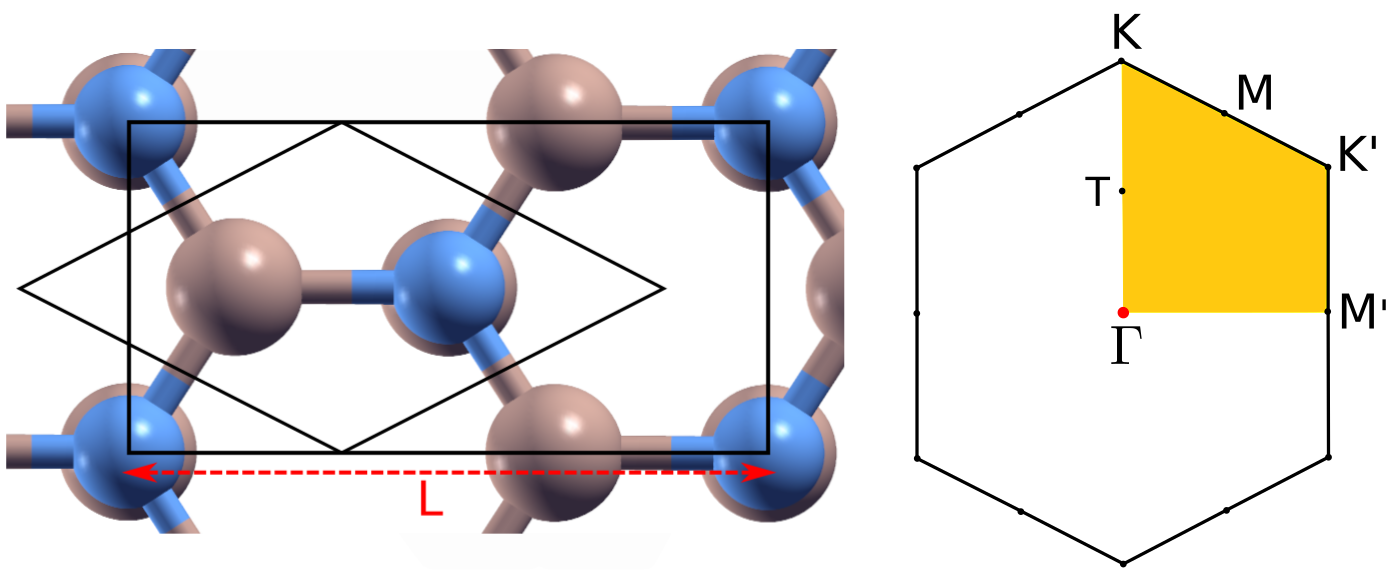
\includegraphics[width=0.5\textwidth]{AppB_structure_BZ.png}
%     \caption{This is Fig. 1 from the main text, put here for convenience.}
% \end{figure}
In our case we a have a crystal with a two-atom basis. We simulate uni-axial strain by elongating or shortening the bond length in only one cartesian direction and letting the atoms relax along the other two orthogonal directions.
It is straightforward to impose such a constraint to a lattice with orthogonal vectors, but more complicated if we had kept the equilibrium hexagonal unit cell. This is why we chose to do the relaxation of structures under strain with orthorombic cells containing 8 atoms (4 per plan).
We want to build a unit cell that preserves the symmetry and periodicity of the strained crystal, with as few atoms as possible. The following is a geometrical generalization of the transformation from orthorombic to hexagonal lattice unit cell in cartesian coordinates.\\
Take an orthorombic unit cell whose matrix in cartesian coordinates is :
\begin{equation}
\begin{pmatrix}
a & 0 & 0\\
0 & b & 0\\
0 & 0 & c
\end{pmatrix}
\end{equation}
with $a,b,c$ being arbitrary lengths.
Now we want to build a strained unit cell that resembles the equilibrium hexagonal cell the most, so that we can compare the different Brillouin zones and the paths on which we plot the electronic structure and the phonon dispersion. The rhombus representing the unit cell of the pseudo-hexagonal cell, viewed from the top, is drawn in Fig. \ref{fig:rhomb}.
\begin{figure}[b]
    \centering
    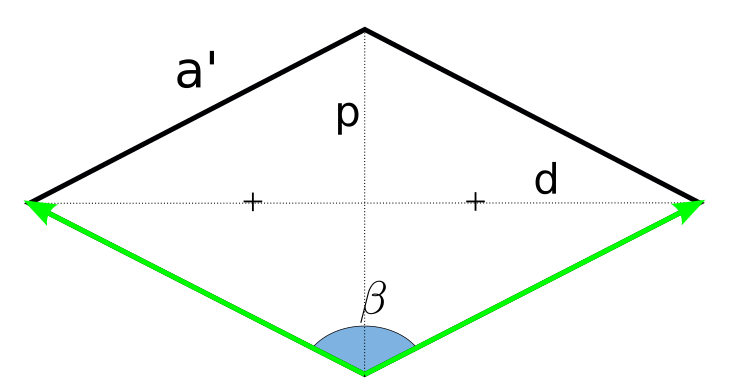
\includegraphics[width=0.5\textwidth]{AppB_rhombus.png}
    \caption{Rhombus used as the unit cell for the pseudo-hexagonal lattice with the atom positions indicated, viewed from top.}
    \label{fig:rhomb}
\end{figure}
Then we have :
\begin{align}
    a' & = \sqrt{d^2 + p^2} \\
    \beta &= \pi - 2 \tan ^{-1} \left(\frac{p}{d}\right)
\end{align}
where $d,p$ are the half diagonals of the rhombus, $a'$ is the side length and $\beta$ the angle as shown in Fig \ref{fig:rhomb}. This is a regular rhombus in the sense that all sides have equal length and the diagonals are orthogonal. The length of the diagonals is obtained from the knowledge of the orthorombic cell, as shown in Fig. \ref{fig:strain_BZ} in the main text.
Then the matrix of this rhombus unit cell, expressed in cartesian coordinates, is :
\begin{equation}
\begin{pmatrix}
a' & 0 & 0\\
a'\cos\beta & a'\sin\beta & 0\\
0 & 0 & c
\end{pmatrix}
\end{equation}
The first two lines are the vectors in green in Fig. \ref{fig:rhomb}. The third vector $c$ is the one perpendicular to the atomic planes and is the same than the orthorombic $c$.
In the equilibrium case, we have $\beta = 120$\textdegree, then this matrix reduces to :
\begin{equation}
\begin{pmatrix}
a' & 0 & 0\\
-a'/2 & a'\sqrt{3}/2 & 0\\
0 & 0 & c
\end{pmatrix}
\end{equation}
which is the standard hexagonal-lattice unit cell. We now have built a 2-atom unit cell which we used to compute electronic, phononic and optical properties of our strained materials. We checked that both the orthorombic and the pseudo-hexagonal unit cells form the same strained crystal when periodically repeated in all directions.
			%% annexes

\end{document}
